% !TeX program = xelatex
% !TeX encoding = utf-8
% ============================================================
% EXECUTIVE CAPABILITY PROFILE & STATEMENT OF QUALIFICATIONS 2026 (12 PAGES)
% CÔNG TY CỔ PHẦN CÔNG NGHỆ XÂY DỰNG TÂN THÀNH CÔNG (TTC JSC)
% TỔNG THẦU EPC CÔNG NGHIỆP XANH & HẠ TẦNG TIÊU CHUẨN ESG
% PHIÊN BẢN ĐỘT PHÁ - CHUẨN QUỐC TẾ & ĐA NGÔN NGỮ
% ============================================================

\documentclass[11pt,a4paper]{article}

% --- GEOMETRY & LAYOUT ---
\usepackage[
  paperwidth=210mm,
  paperheight=297mm,
  left=12mm,
  right=12mm,
  top=14mm,
  bottom=14mm,
  footskip=8mm
]{geometry}

% --- FONTS & VIETNAMESE TYPOGRAPHY ---
\usepackage{fontspec}
\IfFontExistsTF{Segoe UI}{
  \setmainfont{Segoe UI}[
    BoldFont={Segoe UI Bold},
    ItalicFont={Segoe UI Italic},
    BoldItalicFont={Segoe UI Bold Italic}
  ]
  \newfontfamily\titlefont{Segoe UI Semibold}
}{
  \setmainfont{Arial}[
    BoldFont={Arial Bold},
    ItalicFont={Arial Italic},
    BoldItalicFont={Arial Bold Italic}
  ]
  \newfontfamily\titlefont{Arial Bold}
}

% --- GRAPHICS & TIKZ ---
\usepackage{xcolor}
\usepackage{graphicx}
\usepackage{tikz}
\usetikzlibrary{calc,positioning,shapes.geometric,fit,backgrounds,shadows.blur}

% --- TABLES & LAYOUT HELPERS ---
\usepackage{tabularx}
\usepackage{booktabs}
\usepackage{enumitem}
\usepackage[hidelinks,pdfencoding=auto]{hyperref}
\usepackage{parskip}
\usepackage{setspace}
\usepackage{fontawesome5}
\usepackage{calc}

\newcolumntype{Y}{>{\centering\arraybackslash}X}

% --- COLOR PALETTE (TTC LUXURY CORPORATE SYSTEM) ---
\definecolor{TTCDeepNavy}{HTML}{0B294A}  % Royal Deep Navy Blue
\definecolor{TTCBlue}{HTML}{00529C}      % TTC Corporate Brand Blue
\definecolor{TTCRed}{HTML}{E31B23}       % TTC Brand Dynamic Red
\definecolor{TTCCyan}{HTML}{00A3E0}      % ConTech Cyan Accent
\definecolor{TTCLightBlue}{HTML}{F0F5FA} % Premium Card Background
\definecolor{TTCBorder}{HTML}{D0DFEE}    % Clean Modern Border
\definecolor{TTCTextDark}{HTML}{1A2B3C}  % Crisp Typography Dark Slate
\definecolor{TTCGold}{HTML}{D4AF37}      % Luxury Gold Accent
\definecolor{TTCDarkCard}{HTML}{0D3259}  % Darker card background

\pagestyle{empty}

% --- REUSABLE HEADER & FOOTER BARS ---
\newcommand{\pageheaderbar}[2]{%
  \begin{tikzpicture}[remember picture,overlay]
    \fill[TTCDeepNavy] (current page.north west) rectangle ++(\paperwidth,-10mm);
    \draw[TTCRed,line width=1.5pt] ([yshift=-10mm]current page.north west) -- ++(\paperwidth,0);
    \node[anchor=west,text=white,inner sep=0pt] at ([xshift=12mm,yshift=-5mm]current page.north west) {%
      {\fontsize{7.5}{9}\selectfont\bfseries CÔNG TY CỔ PHẦN CÔNG NGHỆ XÂY DỰNG TÂN THÀNH CÔNG | TTC JSC}%
    };
    \node[anchor=east,text=TTCCyan,inner sep=0pt] at ([xshift=-12mm,yshift=-5mm]current page.north east) {%
      {\fontsize{7.5}{9}\selectfont\bfseries #1}%
    };
  \end{tikzpicture}%
  \vspace{1.5mm}%
}

\newcommand{\pagefooterbar}[1]{%
  \begin{tikzpicture}[remember picture,overlay]
    \node[anchor=south,fill=TTCLightBlue,draw=TTCBorder,line width=0.5pt,minimum width=\paperwidth,minimum height=7.5mm,inner sep=0pt] at (current page.south) {};
    \draw[TTCBlue,line width=1.5pt] ([yshift=7.5mm]current page.south west) -- ([yshift=7.5mm]current page.south east);
    \node[anchor=south west,text=TTCTextDark,inner sep=0pt] at ([xshift=12mm,yshift=2.2mm]current page.south west) {%
      {\fontsize{7}{8.5}\selectfont\faPhone\ +84 976 447 766 \quad\textbullet\quad \faEnvelope\ info@tanthanhcongjsc.com \quad\textbullet\quad \faGlobe\ https://tanthanhcongjsc.com \quad\textbullet\quad \faMapMarker*\ Hà Nội, Việt Nam}%
    };
    \node[anchor=south east,text=TTCBlue,inner sep=0pt] at ([xshift=-12mm,yshift=2.2mm]current page.south east) {%
      {\fontsize{7.5}{9}\selectfont\bfseries #1}%
    };
  \end{tikzpicture}%
}

\newcommand{\secbrand}[2]{%
  \vspace{1mm}%
  \noindent{\fontsize{14.5}{17.5}\selectfont\bfseries\color{TTCBlue} #1}\\[-1pt]
  \noindent{\fontsize{8.2}{10.5}\selectfont\itshape\color{TTCCyan} #2}\\[1.5pt]
  {\color{TTCRed}\rule{45mm}{1.5pt}}%
  \vspace{2mm}%
}

\begin{document}

% ============================================================
% TRANG 1: BÌA CHÍNH -- THIẾT KẾ SOQ ĐẲNG CẤP QUỐC TẾ (SANG TRỌNG & ĐỒNG BỘ)
% ============================================================
\begin{tikzpicture}[remember picture,overlay]
  % 1. Full-page background photo (Industrial Factory Construction)
  \node[anchor=center,inner sep=0pt] at (current page.center) {
    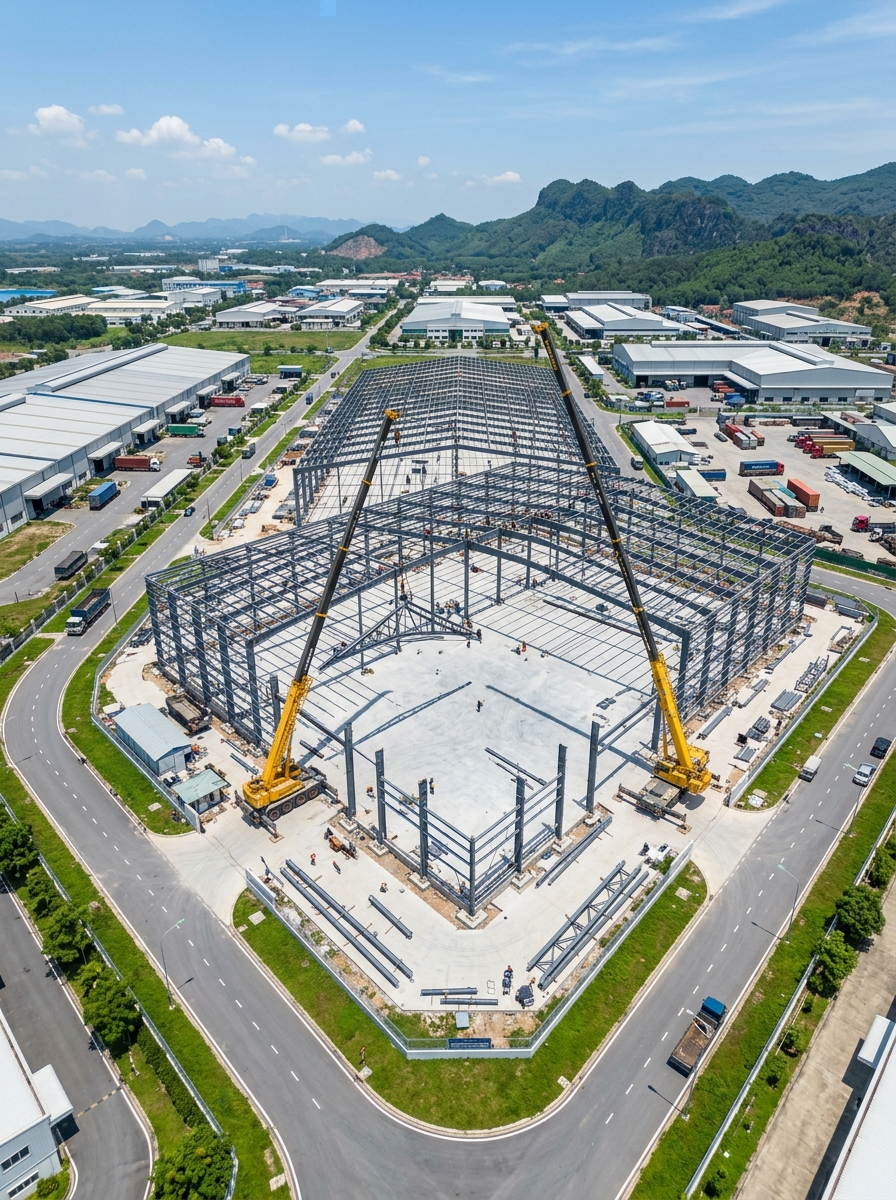
\includegraphics[width=\paperwidth,height=\paperheight]{../../public/executive-cover-hero.jpg}
  };

  % 2. Cohesive Dark Luxury Architectural Overlay (Unified, no harsh striped cuts)
  \shade[
    top color=TTCDeepNavy!96!black,
    middle color=TTCDeepNavy!82!black,
    bottom color=TTCDeepNavy!98!black,
    opacity=0.88
  ] (current page.south west) rectangle (current page.north east);

  % 3. Top Decorative Accent Lines
  \fill[TTCBlue] (current page.north west) rectangle ++(\paperwidth,-4mm);
  \fill[TTCRed] ([yshift=-4mm]current page.north west) rectangle ++(\paperwidth,-1.5mm);

  % 4. Top Corporate Branding Header
  \node[
    anchor=north,
    inner sep=0pt,
    text width=182mm
  ] at ([yshift=-12mm]current page.north) {
    \begin{minipage}{\linewidth}
      \begin{tabularx}{\linewidth}{@{}l X r@{}}
        % Logo in white luxury capsule
        \begin{tikzpicture}[baseline=(logo.center)]
          \node[
            name=logo,
            fill=white,
            rounded corners=4pt,
            inner sep=4pt,
            draw=TTCBorder,
            line width=0.5pt
          ] {
            
\includegraphics[height=13mm]{../../public/logo.png}
          };
        \end{tikzpicture}
        &
        \vspace{1mm}
        {\fontsize{9.5}{12}\selectfont\bfseries\color{white} CÔNG TY CỔ PHẦN CÔNG NGHỆ XÂY DỰNG TÂN THÀNH CÔNG}\newline
        {\fontsize{7.5}{9.5}\selectfont\color{TTCCyan} TAN THANH CONG CONSTRUCTION TECHNOLOGY JOINT STOCK COMPANY}
        &
        
\begin{tikzpicture}[baseline=(tag.center)]
          \node[
            name=tag,
            fill=TTCRed!90!black,
            text=white,
            rounded corners=3pt,
            inner sep=4pt
          ] {
            {\fontsize{7.5}{9}\selectfont\bfseries SOQ 2026 \faLock}
          };
        \end{tikzpicture}
      \end{tabularx}
    \end{minipage}
  };

  % Thin decorative separator line
  \draw[TTCCyan!60!white,line width=0.8pt] ([xshift=14mm,yshift=-34mm]current page.north west) -- ([xshift=-14mm,yshift=-34mm]current page.north east);

  % 5. Hero SOQ Document Title Block (Center-weighted, monumental & prestigious)
  \node[
    anchor=center,
    align=center,
    text width=182mm,
    inner sep=0pt
  ] at ([yshift=38mm]current page.center) {
    {\fontsize{10.5}{13}\selectfont\bfseries\color{TTCCyan} BÁO CÁO NĂNG LỰC TỔNG THẦU EPC \& TIỀN KHẢ THI (SOQ)}\\[6pt]
    {\fontsize{26}{31}\selectfont\bfseries\color{white} EXECUTIVE}\\[1pt]
    {\fontsize{26}{31}\selectfont\bfseries\color{white} CAPABILITY PROFILE}\\[8pt]
    {\color{TTCRed}\rule{60mm}{2.5pt}}\\[8pt]
    {\fontsize{12}{15}\selectfont\bfseries\color{TTCGold} TỔNG THẦU EPC CÔNG NGHIỆP XANH \& HẠ TẦNG TIÊU CHUẨN ESG}\\[4pt]
    {\fontsize{8.5}{11.5}\selectfont\color{white!85!white} Turnkey Industrial EPC General Contractor \quad\textbullet\quad High-Tech PEB \quad\textbullet\quad ConTech Digital Infrastructure}
  };

  % 6. Value Proposition Statement (Clean glass-tinted minimalist ribbon)
  \node[
    anchor=center,
    fill=TTCBlue!40!TTCDeepNavy,
    draw=TTCCyan!50!white,
    line width=0.8pt,
    rounded corners=6pt,
    minimum width=182mm,
    inner sep=8pt,
    text width=172mm,
    align=center
  ] at ([yshift=-15mm]current page.center) {
    {\fontsize{10.5}{13.5}\selectfont\bfseries\color{TTCCyan} “Chất Lượng Vững Bền -- Kỹ Thuật Tiên Phong -- Chuẩn Mực Quốc Tế”}\\[3pt]
    {\fontsize{8.2}{11.5}\selectfont\color{white!92!white}
    Đối tác Tổng thầu EPC một đầu mối đáng tin cậy của 150+ tập đoàn FDI toàn cầu (Nhật Bản, Hàn Quốc, Đài Loan, Châu Âu). Tiên phong kết hợp công nghệ kết cấu thép nhịp lớn cùng giải pháp số hóa ConTech từ hệ sinh thái AIDC.}
  };

  % 7. Key Capability Pillars (4 Balanced Column Cards with Perfect Tabular Alignment)
  \node[
    anchor=south,
    fill=TTCDeepNavy!95!black,
    draw=TTCCyan!60!white,
    line width=1pt,
    rounded corners=6pt,
    minimum width=182mm,
    inner sep=6pt,
    text width=176mm,
    align=center
  ] at ([yshift=24mm]current page.south) {
    \begin{tabularx}{\linewidth}{@{}Y|Y|Y|Y@{}}
      {\fontsize{17}{19}\selectfont\bfseries\color{TTCRed} 10+} &
      {\fontsize{17}{19}\selectfont\bfseries\color{TTCCyan} 150+} &
      {\fontsize{17}{19}\selectfont\bfseries\color{white} >500.000 m²} &
      {\fontsize{17}{19}\selectfont\bfseries\color{TTCGold} 30.000 T} \\
      {\fontsize{7.5}{9}\selectfont\bfseries\color{white} NĂM THỰC CHIẾN} &
      {\fontsize{7.5}{9}\selectfont\bfseries\color{white} DỰ ÁN HOÀN THÀNH} &
      {\fontsize{7.5}{9}\selectfont\bfseries\color{white} SÀN CÔNG NGHIỆP} &
      {\fontsize{7.5}{9}\selectfont\bfseries\color{white} THÉP PEB / NĂM} \\
      {\fontsize{6.5}{8}\selectfont\color{white!70!white} EPC Công nghiệp FDI} &
      {\fontsize{6.5}{8}\selectfont\color{white!70!white} Nhật, Hàn, Đài Loan} &
      {\fontsize{6.5}{8}\selectfont\color{white!70!white} Nhà xưởng \& KCN} &
      {\fontsize{6.5}{8}\selectfont\color{white!70!white} Công suất Nhà máy}
    \end{tabularx}
  };

  % 8. Bottom Authority & Certification Footer Bar
  \fill[TTCBlue] (current page.south west) rectangle ++(\paperwidth,13mm);
  \draw[TTCRed,line width=1.5pt] ([yshift=13mm]current page.south west) -- ++(\paperwidth,0);

  \node[anchor=south,text=white,inner sep=0pt] at ([yshift=4.5mm]current page.south) {
    {\fontsize{7.2}{9}\selectfont
    \faPhone\ +84 976 447 766 \quad\textbullet\quad
    \faEnvelope\ info@tanthanhcongjsc.com \quad\textbullet\quad
    \faGlobe\ https://tanthanhcongjsc.com \quad\textbullet\quad
    \faAward\ NĂNG LỰC HẠNG I BXD \quad\textbullet\quad
    \faCertificate\ ISO 9001 / 14001 / 45001 \quad\textbullet\quad
    \faHandshake\ FIDIC EPC}
  };
\end{tikzpicture}

\newpage

% ============================================================
% TRANG 2: THÔNG ĐIỆP LÃNH ĐẠO & CAM KẾT BẢO LÃNH C-LEVEL
% ============================================================
\pageheaderbar{THÔNG ĐIỆP LÃNH ĐẠO \& CAM KẾT C-LEVEL}{Trang 02}
\pagefooterbar{Trang 02}

\begin{minipage}[t][252mm]{\textwidth}
\secbrand{Thông Điệp Ban Lãnh Đạo \& Cam Kết Trách Nhiệm Cấp Cao}{Executive Accountability Statement \& Corporate Risk Management Governance}

% CEO Message Box
\noindent
\begin{tikzpicture}
  \node[
    rounded corners=6pt, fill=TTCLightBlue, draw=TTCBorder, line width=0.8pt,
    minimum width=186mm, inner sep=8pt, text width=176mm, align=left
  ] {
    {\fontsize{8.5}{12.5}\selectfont\color{TTCTextDark}
    \textit{Kính gửi Quý Chủ tịch, Quý Tổng Giám đốc và Các Trưởng Ban Quản lý Dự án FDI!}\\[2pt]
    Trong bối cảnh dịch chuyển chuỗi cung ứng toàn cầu sang Việt Nam, quyết định chọn Tổng thầu EPC cho tổ hợp nhà máy hàng chục triệu USD là quyết định chiến lược ảnh hưởng trực tiếp đến dòng tiền, thời gian sản xuất và uy tín thương hiệu.\\[3pt]
    {\fontsize{9.5}{13.5}\selectfont\bfseries\color{TTCBlue}
    ``Lòng tin của khách hàng không đến từ lời hứa, mà được khẳng định qua từng liên kết bu lông chính xác, sự an toàn tuyệt đối trên công trường và cam kết bàn giao đúng hẹn.''}\\[3pt]
    TTC không chỉ là nhà thầu thi công -- chúng tôi là \textbf{đối tác chiến lược đồng hành xuyên suốt vòng đời dự án}, từ tư vấn quy hoạch, thiết kế kỹ thuật, sản xuất kết cấu thép đến bàn giao vận hành. Với sự \textbf{bảo trợ công nghệ từ AIDC (Công ty CP Công nghệ AI và Chuyển Đổi Số Việt Nam)}, TTC tiên phong tích hợp giải pháp ConTech thông minh -- tối ưu kết cấu thép bằng thuật toán AI và giám sát an toàn tự động 24/7.}

    \vspace{2.5mm}
    \begin{tabularx}{\linewidth}{@{}p{65mm} X r@{}}
      {\fontsize{9}{11}\selectfont\bfseries\color{TTCRed} PHẠM HUY TÂN} &
      {\fontsize{8}{10}\selectfont\bfseries\color{TTCBlue} \textbullet\quad Tổng Giám đốc / CEO -- TTC JSC} &
      {\fontsize{7.5}{9.5}\selectfont\itshape\color{TTCTextDark} \faAward\ 10+ Năm Điều Hành Hạ Tầng FDI}
    \end{tabularx}
  };
\end{tikzpicture}

\vspace{2mm}

% Middle: Site Photo + 3 Golden Guarantees
\noindent
\begin{tabular}{@{}p{91mm}@{\hspace{4mm}}p{91mm}@{}}
  % Left: Photo
  \begin{tikzpicture}
    \node[rounded corners=6pt, draw=TTCBorder, line width=0.8pt, inner sep=0pt, fill=white] (pimg) {
      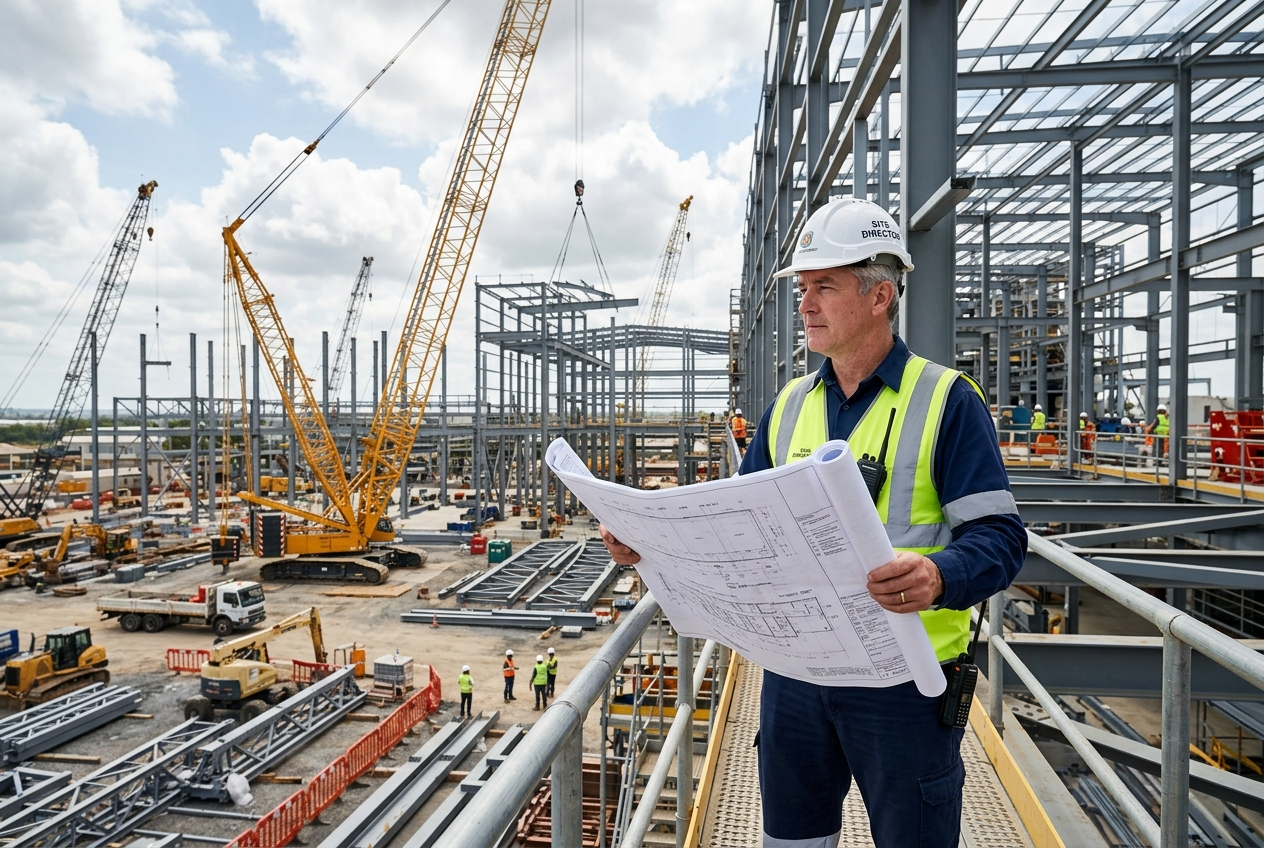
\includegraphics[width=91mm,height=55mm]{../../public/c_level_site_inspection.jpg}
    };
    \node[
      anchor=south, fill=TTCDeepNavy!95!black, draw=TTCCyan!80!white,
      line width=0.6pt, text=white, rounded corners=4pt, inner sep=4pt,
      text width=85mm, align=center
    ] at ([yshift=2mm]pimg.south) {
      {\fontsize{8}{9.5}\selectfont\bfseries\color{TTCCyan} \faAward\ TỔNG THẦU EPC CÔNG NGHIỆP HẠNG I}\\[1.5pt]
      {\fontsize{6.8}{8}\selectfont Chứng chỉ năng lực hoạt động xây dựng cấp bởi Bộ Xây dựng}
    };
  \end{tikzpicture}
  &
  % Right: 3 Guarantees
  \begin{tikzpicture}
    \node[
      rounded corners=6pt, fill=white, draw=TTCBlue!40!white, line width=0.8pt,
      minimum width=91mm, minimum height=55mm, inner sep=6pt, align=left, text width=84mm
    ] {
      {\fontsize{9.5}{11.5}\selectfont\bfseries\color{TTCBlue} \faShield*\quad 3 CAM KẾT BẢO LÃNH EPC}\\[4pt]
      {\fontsize{8}{11.5}\selectfont
      \textbf{\color{TTCRed} \faCheckCircle\ 100\% ON-TIME DELIVERY:}\newline
      Kiểm soát tiến độ CPM \& mô hình 4D BIM, bù tiến độ 3 ca liên tục, cam kết bồi thường hợp đồng nếu chậm trễ.\\[3pt]
      \textbf{\color{TTCRed} \faCheckCircle\ 0\% ACCIDENT -- ZERO HSE:}\newline
      Tiêu chuẩn ISO 45001, 100\% công nhân có thẻ an toàn, PPE chuẩn Châu Âu, diễn tập PCCC định kỳ.\\[3pt]
      \textbf{\color{TTCRed} \faCheckCircle\ VALUE ENGINEERING -15\%:}\newline
      Tối ưu tiết diện kết cấu thép bằng AI, giảm 10--15\% chi phí mà tăng cường độ chịu lực.}
    };
  \end{tikzpicture}
\end{tabular}

\vspace{2mm}

% Strategic Direction 3-column dark banner
\noindent
\begin{tikzpicture}
  \node[
    rounded corners=6pt, fill=TTCDeepNavy!95!black, draw=TTCCyan!80!white, line width=1pt,
    text=white, minimum width=186mm, inner sep=7pt, text width=176mm, align=center
  ] {
    {\fontsize{9.5}{11.5}\selectfont\bfseries\color{TTCRed} \faRocket\quad NĂNG LỰC \& ĐỊNH HƯỚNG CHIẾN LƯỢC}\\[4pt]
    \begin{tabularx}{\linewidth}{@{}p{56mm} p{56mm} X@{}}
      {\fontsize{8.5}{10.5}\selectfont\bfseries\color{TTCCyan} \faBullseye\ SỨ MỆNH} &
      {\fontsize{8.5}{10.5}\selectfont\bfseries\color{TTCCyan} \faEye\ TẦM NHÌN 2030} &
      {\fontsize{8.5}{10.5}\selectfont\bfseries\color{TTCCyan} \faNetworkWired\ MẠNG LƯỚI} \\
      {\fontsize{7.5}{10.5}\selectfont Tổng thầu EPC xanh hàng đầu Việt Nam, dẫn đầu về tiến độ, chất lượng và giải pháp số hóa cho tập đoàn FDI.} &
      {\fontsize{7.5}{10.5}\selectfont Top 10 Tổng thầu xây dựng công nghiệp FDI uy tín, hiện đại và chuẩn mực quốc tế tại Việt Nam.} &
      {\fontsize{7.5}{10.5}\selectfont Đảm nhận đồng thời 10--15 đại công trường Fast-track trên 20+ tỉnh thành công nghiệp cả nước.}
    \end{tabularx}
  };
\end{tikzpicture}

\vspace{2mm}

% Additional differentiator ribbon
\noindent
\begin{tikzpicture}
  \node[
    rounded corners=6pt, fill=TTCBlue, text=white,
    minimum width=186mm, minimum height=20mm, inner sep=4pt
  ] {
    \begin{tabularx}{176mm}{@{}Y|Y|Y|Y@{}}
      {\fontsize{15}{17}\selectfont\bfseries\color{TTCRed} 250 TỶ} &
      {\fontsize{15}{17}\selectfont\bfseries\color{TTCCyan} 100\%} &
      {\fontsize{15}{17}\selectfont\bfseries\color{white} 24 GIỜ} &
      {\fontsize{15}{17}\selectfont\bfseries\color{TTCRed} 0 VNĐ} \\
      {\fontsize{7}{9}\selectfont Hạn mức Bảo lãnh \& Tín dụng} &
      {\fontsize{7}{9}\selectfont Đúng Tiến độ Cam kết} &
      {\fontsize{7}{9}\selectfont Phát hành Thư Bảo lãnh} &
      {\fontsize{7}{9}\selectfont Nợ đọng Thầu phụ}
    \end{tabularx}
  };
\end{tikzpicture}
\end{minipage}

\newpage

% ============================================================
% TRANG 3: TỔNG QUAN PHÁP LÝ & QUY CHUẨN QUỐC TẾ
% ============================================================
\pageheaderbar{TỔNG QUAN DOANH NGHIỆP \& HỒ SƠ PHÁP LÝ}{Trang 03}
\pagefooterbar{Trang 03}

\begin{minipage}[t][252mm]{\textwidth}
\secbrand{Tổng Quan Doanh Nghiệp \& Hồ Sơ Năng Lực Pháp Lý Hạng I}{Corporate Profile, Grade 1 Qualification \& International Engineering Standards}

% Company Info Card
\noindent
\begin{tikzpicture}
  \node[
    rounded corners=6pt, fill=TTCLightBlue, draw=TTCBorder, line width=0.8pt,
    minimum width=186mm, inner sep=7pt, text width=176mm, align=left
  ] {
    {\fontsize{9.5}{11.5}\selectfont\bfseries\color{TTCBlue} \faIdCard\quad THÔNG TIN PHÁP LÝ DOANH NGHIỆP}\\[3pt]
    {\fontsize{8}{12}\selectfont
    \begin{tabularx}{\linewidth}{@{}p{38mm} X p{32mm} X@{}}
      \textbf{Tên doanh nghiệp:} & \multicolumn{3}{l}{\textbf{CÔNG TY CỔ PHẦN CÔNG NGHỆ XÂY DỰNG TÂN THÀNH CÔNG}} \\
      \textbf{Tên quốc tế:} & \multicolumn{3}{l}{TAN THANH CONG CONSTRUCTION TECHNOLOGY JOINT STOCK COMPANY} \\
      \textbf{Mã số thuế / MSDN:} & \textbf{0107090447} (Cấp ngày 10/11/2015) & \textbf{Đại diện pháp luật:} & Ông PHẠM HUY TÂN -- TGĐ \\
      \textbf{Trụ sở ĐKKD:} & \multicolumn{3}{l}{Số 39, ngõ 292 đường Kim Giang, P. Đại Kim, Q. Hoàng Mai, TP. Hà Nội} \\
      \textbf{Văn phòng điều hành:} & \multicolumn{3}{l}{Số 19N7B, KĐT Trung Hòa Nhân Chính, Q. Thanh Xuân, TP. Hà Nội}
    \end{tabularx}}
  };
\end{tikzpicture}

\vspace{2mm}

% 4 Legal Pillars (2x2) -- increased height
\noindent
\begin{tabular}{@{}p{91mm}@{\hspace{4mm}}p{91mm}@{}}
  \begin{tikzpicture}
    \node[
      rounded corners=6pt, fill=white, draw=TTCRed!80!white, line width=1pt,
      minimum width=91mm, minimum height=44mm, inner sep=6pt, align=left, text width=84mm
    ] {
      {\fontsize{9.5}{11.5}\selectfont\bfseries\color{TTCRed} \faAward\ CHỨNG CHỈ NĂNG LỰC HẠNG I (BỘ XÂY DỰNG)}\\[3pt]
      {\fontsize{7.8}{11.2}\selectfont\color{TTCTextDark}
      Đủ điều kiện pháp lý làm \textbf{Tổng thầu EPC thi công công trình Cấp I} quy mô sàn $>100.000$ m² trên toàn quốc. Đảm nhiệm trọn gói: khảo sát hiện trường, thiết kế kỹ thuật, chế tạo kết cấu thép PEB và thi công lắp đặt cơ điện MEP hoàn chỉnh.}
    };
  \end{tikzpicture}
  &
  \begin{tikzpicture}
    \node[
      rounded corners=6pt, fill=white, draw=TTCBlue!40!white, line width=0.8pt,
      minimum width=91mm, minimum height=44mm, inner sep=6pt, align=left, text width=84mm
    ] {
      {\fontsize{9.5}{11.5}\selectfont\bfseries\color{TTCBlue} \faCertificate\ ISO 9001:2015 -- CHẤT LƯỢNG THI CÔNG}\\[3pt]
      {\fontsize{7.8}{11.2}\selectfont\color{TTCTextDark}
      Hệ thống Quản lý Chất lượng chuẩn hóa toàn diện: kiểm tra 100\% vật tư đầu vào có CO/CQ, siêu âm mối hàn UT/MT theo AWS D1.1, nghiệm thu chuyển bước ITP có chữ ký Tư vấn Giám sát quốc tế xác nhận.}
    };
  \end{tikzpicture}
  \\[2mm]
  \begin{tikzpicture}
    \node[
      rounded corners=6pt, fill=white, draw=TTCBlue!40!white, line width=0.8pt,
      minimum width=91mm, minimum height=44mm, inner sep=6pt, align=left, text width=84mm
    ] {
      {\fontsize{9.5}{11.5}\selectfont\bfseries\color{TTCBlue} \faShield*\ ISO 45001:2018 -- AN TOÀN LAO ĐỘNG HSE}\\[3pt]
      {\fontsize{7.8}{11.2}\selectfont\color{TTCTextDark}
      Hệ thống Quản lý An toàn \& Sức khỏe Nghề nghiệp chuẩn quốc tế. Chính sách \textbf{Zero Accident} nghiêm ngặt, 100\% công nhân huấn luyện ATLĐ, kiểm định thiết bị nâng hạ định kỳ, đội ứng cứu khẩn cấp 24/7.}
    };
  \end{tikzpicture}
  &
  \begin{tikzpicture}
    \node[
      rounded corners=6pt, fill=white, draw=TTCBlue!40!white, line width=0.8pt,
      minimum width=91mm, minimum height=44mm, inner sep=6pt, align=left, text width=84mm
    ] {
      {\fontsize{9.5}{11.5}\selectfont\bfseries\color{TTCBlue} \faLeaf\ ISO 14001:2015 -- MÔI TRƯỜNG \& ESG}\\[3pt]
      {\fontsize{7.8}{11.2}\selectfont\color{TTCTextDark}
      Hệ thống Quản lý Môi trường tiên tiến. Giảm thiểu phát thải bụi PM2.5, quản lý 100\% rác thải xây dựng theo quy chuẩn, ưu tiên vật liệu Low-Carbon và tư vấn chứng chỉ công trình xanh LEED/LOTUS/EDGE.}
    };
  \end{tikzpicture}
\end{tabular}

\vspace{2mm}

% International Standards Matrix -- expanded
\noindent
\begin{tikzpicture}
  \node[
    rounded corners=6pt, fill=TTCLightBlue, draw=TTCBorder, line width=0.8pt,
    minimum width=186mm, inner sep=7pt, text width=176mm, align=left
  ] {
    {\fontsize{9}{11}\selectfont\bfseries\color{TTCBlue} \faCogs\quad HỆ QUY CHUẨN KỸ THUẬT \& QUẢN LÝ DỰ ÁN QUỐC TẾ ÁP DỤNG:}\\[3pt]
    {\fontsize{7.5}{11}\selectfont\color{TTCTextDark}
    \textbf{Thiết kế Kết cấu Thép:} AISC 360-16 (Hoa Kỳ), MBMA 2010 (Hiệp hội Nhà thép tiền chế Mỹ), Eurocode 3 (Châu Âu), TCVN 5575:2012.\\
    \textbf{Gia công \& Hàn kết cấu:} AWS D1.1 (Hiệp hội Hàn Hoa Kỳ), ASTM A36 / A572 / SS400 / Q345B, ISO 8501-1 Sa 2.5.\\
    \textbf{Quản trị Hợp đồng EPC:} FIDIC Silver Book / Yellow Book EPC Turnkey, Luật Xây dựng 50/2014/QH13.\\
    \textbf{Thiết kế Nền móng:} TCVN 10304:2014 (Cọc khoan nhồi), BS EN 1997 (Eurocode 7), AS 2159 (Úc).}
  };
\end{tikzpicture}

\vspace{2mm}

% Bottom certification badges ribbon
\noindent
\begin{tikzpicture}
  \node[
    rounded corners=6pt, fill=TTCDeepNavy!95!black, draw=TTCCyan!80!white, line width=1pt,
    text=white, minimum width=186mm, minimum height=22mm, inner sep=4pt
  ] {
    \begin{tabularx}{176mm}{@{}Y|Y|Y|Y|Y@{}}
      {\fontsize{12}{14}\selectfont\bfseries\color{TTCRed} HẠNG I} &
      {\fontsize{12}{14}\selectfont\bfseries\color{TTCCyan} ISO 9001} &
      {\fontsize{12}{14}\selectfont\bfseries\color{white} ISO 45001} &
      {\fontsize{12}{14}\selectfont\bfseries\color{TTCCyan} ISO 14001} &
      {\fontsize{12}{14}\selectfont\bfseries\color{TTCGold} FIDIC} \\
      {\fontsize{7}{8.5}\selectfont Bộ Xây dựng} &
      {\fontsize{7}{8.5}\selectfont Chất lượng} &
      {\fontsize{7}{8.5}\selectfont An toàn HSE} &
      {\fontsize{7}{8.5}\selectfont Môi trường} &
      {\fontsize{7}{8.5}\selectfont EPC Turnkey}
    \end{tabularx}
  };
\end{tikzpicture}
\end{minipage}

\newpage

% ============================================================
% TRANG 4: SƠ ĐỒ TỔ CHỨC & NĂNG LỰC NHÂN SỰ
% ============================================================
\pageheaderbar{SƠ ĐỒ TỔ CHỨC \& ĐỘI NGŨ NHÂN SỰ}{Trang 04}
\pagefooterbar{Trang 04}

\begin{minipage}[t][252mm]{\textwidth}
\secbrand{Sơ Đồ Bộ Máy Vận Hành EPC \& Đội Ngũ Nhân Sự Chuyên Gia}{Organizational Structure, Key Personnel Qualifications \& Human Capital}

% Org Chart
\begin{center}
\begin{tikzpicture}
  \draw[rounded corners=6pt, fill=white, draw=TTCBlue!40!white, line width=0.8pt] (-90mm,-38mm) rectangle (90mm,34mm);

  % Root BOD
  \node[
    rounded corners=4pt, fill=TTCRed, text=white, align=center, inner sep=4pt,
    font=\fontsize{8}{10}\selectfont\bfseries, minimum width=80mm, minimum height=8.5mm
  ] (bod) at (0, 23mm) {
    \faUsers\ HỘI ĐỒNG QUẢN TRỊ \& BAN TỔNG GIÁM ĐỐC\\[1pt]
    {\fontsize{6.8}{8}\selectfont\normalfont Điều hành Chiến lược \& Cam kết Cấp cao C-Level}
  };

  % 4 Departments
  \node[rounded corners=3pt, fill=TTCBlue, text=white, align=center, inner sep=3.5pt,
    font=\fontsize{7.2}{8.8}\selectfont\bfseries, minimum width=41mm, minimum height=7.5mm
  ] (c1) at (-63mm, 9mm) {\faDraftingCompass\ KHỐI KỸ THUẬT \& BIM};

  \node[rounded corners=3pt, fill=TTCBlue, text=white, align=center, inner sep=3.5pt,
    font=\fontsize{7.2}{8.8}\selectfont\bfseries, minimum width=41mm, minimum height=7.5mm
  ] (c2) at (-21mm, 9mm) {\faIndustry\ KHỐI DỰ ÁN \& THI CÔNG};

  \node[rounded corners=3pt, fill=TTCBlue, text=white, align=center, inner sep=3.5pt,
    font=\fontsize{7.2}{8.8}\selectfont\bfseries, minimum width=41mm, minimum height=7.5mm
  ] (c3) at (21mm, 9mm) {\faCogs\ KHỐI MUA SẮM \& PEB};

  \node[rounded corners=3pt, fill=TTCBlue, text=white, align=center, inner sep=3.5pt,
    font=\fontsize{7.2}{8.8}\selectfont\bfseries, minimum width=41mm, minimum height=7.5mm
  ] (c4) at (63mm, 9mm) {\faChartLine\ KHỐI TÀI CHÍNH \& HĐ};

  % Connections
  \draw[TTCBlue, line width=1pt] (bod.south) -- (0, 15mm);
  \draw[TTCBlue, line width=1pt] (-63mm, 15mm) -- (63mm, 15mm);
  \draw[TTCBlue, line width=1pt] (-63mm, 15mm) -- (c1.north);
  \draw[TTCBlue, line width=1pt] (-21mm, 15mm) -- (c2.north);
  \draw[TTCBlue, line width=1pt] (21mm, 15mm) -- (c3.north);
  \draw[TTCBlue, line width=1pt] (63mm, 15mm) -- (c4.north);

  % Detail subnodes -- deeper content
  \node[rounded corners=3pt, fill=TTCLightBlue, draw=TTCBorder, line width=0.6pt,
    align=left, inner sep=3.5pt, font=\fontsize{6.8}{9}\selectfont, text width=37mm, anchor=north
  ] at (-63mm, 4.5mm) {
    \textbullet\ Phòng Thiết kế Kết cấu thép\newline
    \textbullet\ Phòng Cơ điện MEP\newline
    \textbullet\ Trung tâm Số hóa BIM 3D/4D\newline
    \textbullet\ R\&D Công nghệ AI (AIDC)\newline
    \textbullet\ Giám sát Chất lượng Vật liệu
  };

  \node[rounded corners=3pt, fill=TTCLightBlue, draw=TTCBorder, line width=0.6pt,
    align=left, inner sep=3.5pt, font=\fontsize{6.8}{9}\selectfont, text width=37mm, anchor=north
  ] at (-21mm, 4.5mm) {
    \textbullet\ Ban Chỉ huy Công trường\newline
    \textbullet\ Ban QA/QC Chất lượng\newline
    \textbullet\ Ban An toàn HSE độc lập\newline
    \textbullet\ Đội Lắp dựng PEB chuyên sâu\newline
    \textbullet\ Đội Cẩu \& Vận hành Cơ giới
  };

  \node[rounded corners=3pt, fill=TTCLightBlue, draw=TTCBorder, line width=0.6pt,
    align=left, inner sep=3.5pt, font=\fontsize{6.8}{9}\selectfont, text width=37mm, anchor=north
  ] at (21mm, 4.5mm) {
    \textbullet\ Quản lý Chuỗi cung ứng Tier-1\newline
    \textbullet\ Quản lý Xưởng gia công PEB\newline
    \textbullet\ Đấu thầu \& Quản lý Thầu phụ\newline
    \textbullet\ Kiểm định Vật tư CO/CQ\newline
    \textbullet\ Logistics \& Vận chuyển siêu trường
  };

  \node[rounded corners=3pt, fill=TTCLightBlue, draw=TTCBorder, line width=0.6pt,
    align=left, inner sep=3.5pt, font=\fontsize{6.8}{9}\selectfont, text width=37mm, anchor=north
  ] at (63mm, 4.5mm) {
    \textbullet\ Quản trị Dòng tiền Dự án\newline
    \textbullet\ Kế toán Chi phí 5D BIM\newline
    \textbullet\ Quản lý Hợp đồng FIDIC\newline
    \textbullet\ Hạn mức Tín dụng ACB/TPB\newline
    \textbullet\ Pháp chế \& Bảo lãnh Ngân hàng
  };
\end{tikzpicture}
\end{center}

\vspace{2mm}

% HR Stats Banner
\noindent
\begin{tikzpicture}
  \node[
    rounded corners=6pt, fill=TTCBlue, text=white,
    minimum width=186mm, minimum height=24mm, inner sep=4pt
  ] {
    \begin{tabularx}{176mm}{@{}Y|Y|Y|Y@{}}
      {\fontsize{16}{18}\selectfont\bfseries\color{TTCRed} 150+} &
      {\fontsize{16}{18}\selectfont\bfseries\color{TTCCyan} 100\%} &
      {\fontsize{16}{18}\selectfont\bfseries\color{white} 800+} &
      {\fontsize{16}{18}\selectfont\bfseries\color{TTCRed} 10--15} \\
      {\fontsize{7.8}{9}\selectfont Cán bộ Kỹ sư Cơ hữu} &
      {\fontsize{7.8}{9}\selectfont Chỉ huy trưởng Hạng I} &
      {\fontsize{7.8}{9}\selectfont Công nhân Kỹ thuật Lành nghề} &
      {\fontsize{7.8}{9}\selectfont Năm Kinh nghiệm FDI Thực chiến}
    \end{tabularx}
  };
\end{tikzpicture}

\vspace{2mm}

% Key Personnel -- 2 cards expanded
\noindent
\begin{tabular}{@{}p{91mm}@{\hspace{4mm}}p{91mm}@{}}
  \begin{tikzpicture}
    \node[rounded corners=6pt, fill=TTCLightBlue, draw=TTCBorder, line width=0.8pt, minimum width=91mm, minimum height=44mm, inner sep=6pt, align=left, text width=84mm] {
      {\fontsize{9.5}{11.5}\selectfont\bfseries\color{TTCBlue} \faGraduationCap\ NĂNG LỰC CHỈ HUY TRƯỞNG \& THIẾT KẾ}\\[3pt]
      {\fontsize{7.8}{11.2}\selectfont\color{TTCTextDark}
      100\% Giám đốc Dự án và Chỉ huy trưởng tốt nghiệp ĐH Xây dựng, Kiến trúc; chứng chỉ hành nghề Hạng I Bộ Xây dựng. Kinh nghiệm thực chiến điều hành dự án Fast-track vốn FDI Nhật, Hàn, Đài Loan. Thông thạo quy trình nghiệm thu \& quản lý hợp đồng FIDIC quốc tế.}
    };
  \end{tikzpicture}
  &
  \begin{tikzpicture}
    \node[rounded corners=6pt, fill=TTCLightBlue, draw=TTCBorder, line width=0.8pt, minimum width=91mm, minimum height=44mm, inner sep=6pt, align=left, text width=84mm] {
      {\fontsize{9.5}{11.5}\selectfont\bfseries\color{TTCBlue} \faUserShield\ VĂN HÓA AN TOÀN \& ĐÀO TẠO ĐỊNH KỲ}\\[3pt]
      {\fontsize{7.8}{11.2}\selectfont\color{TTCTextDark}
      100\% Kỹ sư và Công nhân hiện trường cấp thẻ an toàn, kiểm tra sức khỏe định kỳ, diễn tập PCCC và cứu hộ trước khi thi công lắp dựng trên cao. Họp giao ban Toolbox Meeting 15 phút mỗi ca -- phổ biến mối nguy và biện pháp an toàn theo từng công đoạn cụ thể.}
    };
  \end{tikzpicture}
\end{tabular}
\end{minipage}

\newpage

% ============================================================
% TRANG 5: BÁO CÁO NĂNG LỰC TÀI CHÍNH & BẢO LÃNH NGÂN HÀNG
% ============================================================
\pageheaderbar{NĂNG LỰC TÀI CHÍNH \& ĐỐI TÁC NGÂN HÀNG}{Trang 05}
\pagefooterbar{Trang 05}

\begin{minipage}[t][252mm]{\textwidth}
\secbrand{Năng Lực Tài Chính Minh Bạch \& Hệ Thống Bảo Lãnh Ngân Hàng}{Financial Solvency, Audited Accounts \& Strategic Banking Credit Facilities}

% Financial Table
\noindent
\begin{tikzpicture}
  \node[
    rounded corners=6pt, fill=white, draw=TTCBlue!40!white, line width=0.8pt,
    minimum width=186mm, inner sep=6pt, text width=176mm, align=center
  ] {
    {\fontsize{9.5}{11.5}\selectfont\bfseries\color{TTCBlue} \faChartLine\quad TÓM TẮT BÁO CÁO TÀI CHÍNH KIỂM TOÁN 3 NĂM GẦN NHẤT}\\[4pt]
    {\fontsize{7.8}{11.2}\selectfont
    \begin{tabularx}{\linewidth}{@{}X c c c@{}}
      \toprule
      \textbf{Chỉ Tiêu Tài Chính (Đơn vị: Tỷ VNĐ)} & \textbf{Năm 2023} & \textbf{Năm 2024} & \textbf{Năm 2025 (KT)} \\
      \midrule
      \textbf{Tổng Tài sản (Total Assets)} & BCTC Kiểm toán & BCTC Kiểm toán & Tăng trưởng vững chắc \\
      \textbf{Vốn Chủ sở hữu (Owner's Equity)} & BCTC Kiểm toán & BCTC Kiểm toán & Đảm bảo an toàn vốn \\
      \textbf{Doanh thu thuần (Net Revenue)} & BCTC Kiểm toán & BCTC Kiểm toán & Tăng trưởng liên tục \\
      \textbf{Lợi nhuận sau thuế (NPAT)} & BCTC Kiểm toán & BCTC Kiểm toán & Lợi nhuận dương ổn định \\
      \textbf{Hệ số Thanh toán (Current Ratio)} & $>1.55$ lần & $>1.65$ lần & \textbf{$>1.85$ lần} \\
      \textbf{Nợ đọng Thầu phụ \& NCC} & \textbf{0 VNĐ} & \textbf{0 VNĐ} & \textbf{0 VNĐ (Cam kết 100\%)} \\
      \bottomrule
    \end{tabularx}}
  };
\end{tikzpicture}

\vspace{2mm}

% 6 Partner Banks
\noindent
\begin{tikzpicture}
  \node[
    rounded corners=6pt, fill=TTCLightBlue, draw=TTCBlue!50!white, line width=0.8pt,
    minimum width=186mm, inner sep=7pt, text width=176mm, align=left
  ] {
    {\fontsize{9.5}{11.5}\selectfont\bfseries\color{TTCBlue} \faUniversity\quad HỆ THỐNG 6 NGÂN HÀNG HỢP TÁC CHIẾN LƯỢC}\\[3pt]
    {\fontsize{8}{12}\selectfont\color{TTCTextDark}
    \textbf{Ngân hàng giao dịch chính:} \textbf{\color{TTCRed}ACB (Ngân hàng TMCP Á Châu)} -- Đối tác chiến lược cấp hạn mức tín dụng lưu động, bảo lãnh dự thầu \& tạm ứng hợp đồng, quản lý dòng tiền dự án chính thức.\\[2pt]
    \textbf{Hệ thống ngân hàng đồng hành:} \textbf{TPBank}, \textbf{Vietcombank (VCB)}, \textbf{BIDV}, \textbf{VietinBank (CTG)}, \textbf{MB Bank} -- sẵn sàng phát hành đa dạng công cụ bảo lãnh: Performance Bond, Advance Payment Guarantee, Warranty Bond.}
  };
\end{tikzpicture}

\vspace{2mm}

% Credit KPI Banner
\noindent
\begin{tikzpicture}
  \node[
    rounded corners=6pt, fill=TTCDeepNavy!95!black, draw=TTCCyan!80!white, line width=1pt,
    text=white, minimum width=186mm, minimum height=26mm, inner sep=4pt
  ] {
    \begin{tabularx}{176mm}{@{}Y|Y|Y@{}}
      {\fontsize{16}{18}\selectfont\bfseries\color{TTCRed} 250 TỶ} &
      {\fontsize{16}{18}\selectfont\bfseries\color{TTCCyan} 100\%} &
      {\fontsize{16}{18}\selectfont\bfseries\color{white} 24 GIỜ} \\
      {\fontsize{7.8}{9.2}\selectfont Hạn mức Bảo lãnh Thầu \& Tín dụng} &
      {\fontsize{7.8}{9.2}\selectfont Sẵn sàng Bảo lãnh Dự thầu \& Tạm ứng} &
      {\fontsize{7.8}{9.2}\selectfont Thời gian Phát hành Thư Bảo lãnh}
    \end{tabularx}
  };
\end{tikzpicture}

\vspace{2mm}

% Financial Strength Notes -- expanded with more detail
\noindent
\begin{tabular}{@{}p{91mm}@{\hspace{4mm}}p{91mm}@{}}
  \begin{tikzpicture}
    \node[rounded corners=6pt, fill=white, draw=TTCBorder, line width=0.8pt, minimum width=91mm, minimum height=42mm, inner sep=6pt, align=left, text width=84mm] {
      {\fontsize{9}{11}\selectfont\bfseries\color{TTCBlue} \faMoneyBillWave\ DÒNG TIỀN VẬN HÀNH DỰ ÁN}\\[2pt]
      {\fontsize{7.5}{11}\selectfont\color{TTCTextDark}
      Nguồn vốn tự có kết hợp hạn mức tín dụng ngân hàng cam kết đảm bảo duy trì mua sắm vật tư, chế tạo kết cấu thép liên tục ngay cả khi Chủ đầu tư chưa kịp giải ngân. TTC cam kết \textbf{không bao giờ để công trường dừng do thiếu dòng tiền} -- đây là nguyên tắc bất khả xâm phạm.}
    };
  \end{tikzpicture}
  &
  \begin{tikzpicture}
    \node[rounded corners=6pt, fill=white, draw=TTCBorder, line width=0.8pt, minimum width=91mm, minimum height=42mm, inner sep=6pt, align=left, text width=84mm] {
      {\fontsize{9}{11}\selectfont\bfseries\color{TTCBlue} \faHandshake\ UY TÍN THANH TOÁN 100\%}\\[2pt]
      {\fontsize{7.5}{11}\selectfont\color{TTCTextDark}
      Lịch sử tín dụng chuẩn mực Nhóm 1 tại Trung tâm Thông tin Tín dụng Quốc gia (CIC), đảm bảo không xảy ra tranh chấp tài chính làm gián đoạn tiến độ. TTC thanh toán \textbf{100\% đúng hạn cho thầu phụ và nhà cung cấp} -- tạo nền tảng uy tín để huy động lực lượng thi công nhanh chóng.}
    };
  \end{tikzpicture}
\end{tabular}

\vspace{2mm}

% Bottom: additional insurance/bonding info
\noindent
\begin{tikzpicture}
  \node[
    rounded corners=6pt, fill=TTCLightBlue, draw=TTCBorder, line width=0.8pt,
    minimum width=186mm, inner sep=6pt, text width=176mm, align=left
  ] {
    {\fontsize{9}{11}\selectfont\bfseries\color{TTCBlue} \faShield*\quad BẢO HIỂM CÔNG TRÌNH \& TRÁCH NHIỆM DÂN SỰ}\\[2pt]
    {\fontsize{7.5}{11}\selectfont\color{TTCTextDark}
    Mua bảo hiểm Mọi Rủi Ro Xây Dựng (CAR Insurance) trị giá tương đương giá trị hợp đồng cho 100\% công trình, bảo hiểm trách nhiệm dân sự với bên thứ ba và bảo hiểm tai nạn lao động cho toàn bộ nhân sự hiện trường theo quy định pháp luật Việt Nam.}
  };
\end{tikzpicture}
\end{minipage}

\newpage

% ============================================================
% TRANG 6: HỆ THỐNG NHÀ XƯỞNG SẢN XUẤT & THIẾT BỊ CƠ GIỚI
% ============================================================
\pageheaderbar{NĂNG LỰC SẢN XUẤT PEB \& THIẾT BỊ THI CÔNG}{Trang 06}
\pagefooterbar{Trang 06}

\begin{minipage}[t][252mm]{\textwidth}
\secbrand{Năng Lực Gia Công Kết Cấu Thép \& Thiết Bị Cơ Giới Hiện Đại}{PEB Steel Structure Manufacturing Capacity \& Heavy Construction Machinery Fleet}

% PEB Capacity
\noindent
\begin{tikzpicture}
  \node[
    rounded corners=6pt, fill=TTCLightBlue, draw=TTCBlue!40!white, line width=0.8pt,
    minimum width=186mm, inner sep=7pt, text width=176mm, align=left
  ] {
    {\fontsize{9.5}{11.5}\selectfont\bfseries\color{TTCBlue} \faIndustry\quad TỔ HỢP NHÀ MÁY GIA CÔNG KẾT CẤU THÉP TIỀN CHẾ (PEB)}\\[3pt]
    {\fontsize{8}{12}\selectfont\color{TTCTextDark}
    \textbf{Công suất gia công:} \textbf{\color{TTCRed}25.000 -- 30.000 Tấn Thép/Năm} (đáp ứng đồng thời 10--15 dự án lớn).\\
    \textbf{Dây chuyền công nghệ:} Máy cắt CNC Plasma Hypertherm ($\pm 0.5$mm), máy gá đính dầm tự động, máy hàn hồ quang chìm SAW (ngấu sâu, ít xỉ), buồng phun bi làm sạch bề mặt thép chuẩn SA 2.5 theo ISO 8501-1, buồng sơn sấy nhiệt công nghiệp Jotun.\\
    \textbf{Kiểm soát chất lượng xưởng:} 100\% phôi thép có Mill Test Certificate (MTC), kiểm tra siêu âm UT mối hàn chịu lực theo AWS D1.1, kéo nén mẫu tại Lab Las-XD, kiểm định nghiệm thu trước khi xuất xưởng.}
  };
\end{tikzpicture}

\vspace{2mm}

% 2 Photo Columns
\noindent
\begin{tabular}{@{}p{91mm}@{\hspace{4mm}}p{91mm}@{}}
  \begin{tikzpicture}
    \node[rounded corners=6pt, draw=TTCBorder, line width=0.8pt, inner sep=0pt, fill=white] (img1) {
      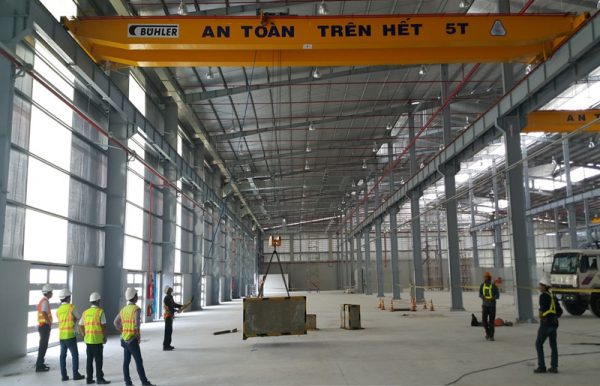
\includegraphics[width=91mm,height=50mm]{../../public/introsection1.jpg}
    };
    \node[anchor=south, fill=TTCBlue!95!black, text=white, rounded corners=4pt, inner sep=3pt, text width=85mm, align=center] at ([yshift=2mm]img1.south) {
      {\fontsize{7.5}{9}\selectfont\bfseries\color{TTCCyan} DÂY CHUYỀN SẢN XUẤT KẾT CẤU THÉP CNC TỰ ĐỘNG}
    };
  \end{tikzpicture}
  &
  \begin{tikzpicture}
    \node[rounded corners=6pt, draw=TTCBorder, line width=0.8pt, inner sep=0pt, fill=white] (img2) {
      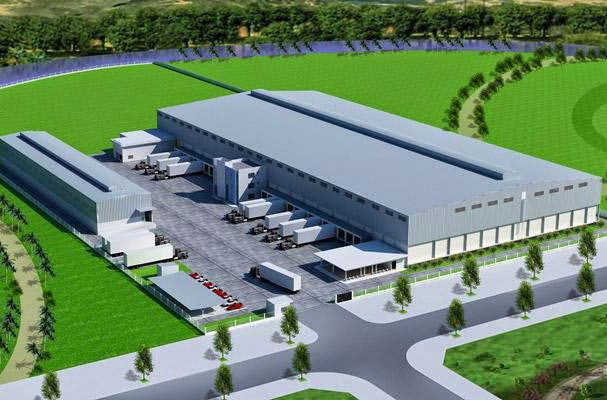
\includegraphics[width=91mm,height=50mm]{../../public/introsection2.jpg}
    };
    \node[anchor=south, fill=TTCBlue!95!black, text=white, rounded corners=4pt, inner sep=3pt, text width=85mm, align=center] at ([yshift=2mm]img2.south) {
      {\fontsize{7.5}{9}\selectfont\bfseries\color{TTCCyan} THI CÔNG LẮP DỰNG KHUNG KÈO KHẨU ĐỘ LỚN AN TOÀN}
    };
  \end{tikzpicture}
\end{tabular}

\vspace{2mm}

% Heavy Equipment Table
\noindent
\begin{tikzpicture}
  \node[
    rounded corners=6pt, fill=white, draw=TTCBorder, line width=0.8pt,
    minimum width=186mm, inner sep=6pt, text width=176mm, align=center
  ] {
    {\fontsize{9.5}{11.5}\selectfont\bfseries\color{TTCBlue} \faTruckLoading\quad DANH MỤC THIẾT BỊ CƠ GIỚI \& XE MÁY CHUYÊN DỤNG}\\[3pt]
    {\fontsize{7.8}{10.8}\selectfont
    \begin{tabularx}{\linewidth}{@{}p{42mm} p{28mm} p{30mm} X@{}}
      \toprule
      \textbf{Chủng loại Thiết bị} & \textbf{Số lượng sở hữu} & \textbf{Thông số Kỹ thuật} & \textbf{Ứng dụng chính} \\
      \midrule
      \textbf{Cẩu tự hành / Cẩu lốp} & 08 Chiếc & 25T -- 100T & Lắp dựng kết cấu thép khẩu độ 36m--60m \\
      \textbf{Máy cán tôn Seamlock di động} & 04 Dàn máy & Cán tại chỗ 100m & Lợp mái không mối nối, chống dột \\
      \textbf{Xe nâng người Boom/Scissor} & 16 Chiếc & 12m -- 28m & Lắp dựng trên cao chuẩn an toàn HSE \\
      \textbf{Máy toàn đạc Laser Leica} & 08 Bộ & $\pm 1$mm & Định vị tim trục, kiểm tra độ thẳng cột \\
      \textbf{Máy hàn SAW tự động} & 12 Bộ & Dòng hàn 600--1000A & Hàn dầm cột chịu lực tại xưởng PEB \\
      \bottomrule
    \end{tabularx}}
  };
\end{tikzpicture}

\vspace{2mm}

% Bottom Equipment Ribbon
\noindent
\begin{tikzpicture}
  \node[
    rounded corners=6pt, fill=TTCDeepNavy!95!black, draw=TTCCyan!80!white, line width=1pt,
    text=white, minimum width=186mm, minimum height=22mm, inner sep=4pt
  ] {
    \begin{tabularx}{176mm}{@{}Y|Y|Y|Y@{}}
      {\fontsize{14}{16}\selectfont\bfseries\color{TTCRed} >150 TỶ VNĐ} &
      {\fontsize{14}{16}\selectfont\bfseries\color{TTCCyan} $\pm 0.5$ mm} &
      {\fontsize{14}{16}\selectfont\bfseries\color{white} 100M LIỀN DẢI} &
      {\fontsize{14}{16}\selectfont\bfseries\color{TTCRed} SA 2.5 ISO} \\
      {\fontsize{7.5}{9}\selectfont Giá trị Đội Cơ giới} &
      {\fontsize{7.5}{9}\selectfont Dung sai Gia công CNC} &
      {\fontsize{7.5}{9}\selectfont Cán Tôn Mái Seamlock} &
      {\fontsize{7.5}{9}\selectfont Tiêu chuẩn Làm sạch Thép}
    \end{tabularx}
  };
\end{tikzpicture}
\end{minipage}

\newpage

% ============================================================
% TRANG 7: CHUỖI GIÁ TRỊ TỔNG THẦU EPC KHÉP KÍN
% ============================================================
\pageheaderbar{CHUỖI GIÁ TRỊ TỔNG THẦU EPC TÍCH HỢP}{Trang 07}
\pagefooterbar{Trang 07}

\begin{minipage}[t][252mm]{\textwidth}
\secbrand{Chuỗi Giá Trị EPC Tích Hợp \& Quy Trình 6 Bước Khép Kín}{Integrated Single-Point Responsibility EPC Roadmap \& 6-Phase Execution Framework}

% Value Statement
\noindent
\begin{tikzpicture}
  \node[
    rounded corners=6pt, fill=TTCLightBlue, draw=TTCBorder, line width=0.8pt,
    minimum width=186mm, inner sep=7pt, text width=176mm, align=left
  ] {
    {\fontsize{8.5}{12}\selectfont\color{TTCTextDark}
    Mô hình \textbf{Tổng thầu EPC một đầu mối (Single-Point Responsibility)} của TTC loại bỏ hoàn toàn trung gian, cho phép Chủ đầu tư chỉ giao dịch với \textbf{một đầu mối duy nhất} từ khảo sát đến bàn giao vận hành -- giúp kiểm soát 100\% chất lượng, \textbf{rút ngắn 30\% tiến độ} và \textbf{tiết kiệm 10--15\% ngân sách} so với tách thầu truyền thống.}
  };
\end{tikzpicture}

\vspace{2mm}

% 6 Steps (2x3) -- increased height to 40mm each
\noindent
\begin{tabular}{@{}p{91mm}@{\hspace{4mm}}p{91mm}@{}}
  \begin{tikzpicture}
    \node[rounded corners=5pt, fill=white, draw=TTCBorder, line width=0.8pt, minimum width=91mm, minimum height=40mm, inner sep=6pt, align=left, text width=84mm] {
      {\fontsize{9.5}{11.5}\selectfont\bfseries\color{TTCRed} \faUsersCog\ 01. TƯ VẤN QUY HOẠCH \& PHÁP LÝ FDI}\\[2.5pt]
      {\fontsize{7.8}{11}\selectfont\color{TTCTextDark}
      Khảo sát địa chất 3D hiện trường, quy hoạch tổng mặt bằng 1/500 tối ưu luồng xe tải và container. Đồng hành trọn gói xin cấp IRC, ERC, ĐTM và thẩm duyệt PCCC trong \textbf{30--45 ngày}. Tư vấn lựa chọn KCN phù hợp nhất về hạ tầng và ưu đãi thuế.}
    };
  \end{tikzpicture}
  &
  \begin{tikzpicture}
    \node[rounded corners=5pt, fill=white, draw=TTCBorder, line width=0.8pt, minimum width=91mm, minimum height=40mm, inner sep=6pt, align=left, text width=84mm] {
      {\fontsize{9.5}{11.5}\selectfont\bfseries\color{TTCBlue} \faDraftingCompass\ 02. THIẾT KẾ KỸ THUẬT \& BIM 3D}\\[2.5pt]
      {\fontsize{7.8}{11}\selectfont\color{TTCTextDark}
      Tối ưu Value Engineering giảm 10--15\% chi phí kết cấu thép, rà soát xung đột Zero-Clash giữa kết cấu và MEP, bóc tách dự toán 5D BIM chính xác từng bu lông, triệt tiêu 100\% chi phí phát sinh ngoài hợp đồng.}
    };
  \end{tikzpicture}
  \\[2mm]
  \begin{tikzpicture}
    \node[rounded corners=5pt, fill=white, draw=TTCBorder, line width=0.8pt, minimum width=91mm, minimum height=40mm, inner sep=6pt, align=left, text width=84mm] {
      {\fontsize{9.5}{11.5}\selectfont\bfseries\color{TTCBlue} \faIndustry\ 03. SẢN XUẤT KẾT CẤU THÉP PEB}\\[2.5pt]
      {\fontsize{7.8}{11}\selectfont\color{TTCTextDark}
      Gia công tự động tại xưởng PEB hiện đại, kiểm định 100\% phôi thép Q345B có MTC, siêu âm đường hàn UT theo AWS D1.1, phun bi Sa 2.5 và sơn 3 lớp Jotun. Công suất \textbf{25.000--30.000 tấn/năm}, đáp ứng Fast-track.}
    };
  \end{tikzpicture}
  &
  \begin{tikzpicture}
    \node[rounded corners=5pt, fill=white, draw=TTCBorder, line width=0.8pt, minimum width=91mm, minimum height=40mm, inner sep=6pt, align=left, text width=84mm] {
      {\fontsize{9.5}{11.5}\selectfont\bfseries\color{TTCBlue} \faBuilding\ 04. THI CÔNG MÓNG \& LẮP DỰNG KHUNG}\\[2.5pt]
      {\fontsize{7.8}{11}\selectfont\color{TTCTextDark}
      Ép cọc bê tông ly tâm D400--D500, đổ bê tông sàn xoa Hardener/Mastertop chịu tải \textbf{10 tấn/m²} cho xe nâng hàng hạng nặng. Cẩu lắp khung kèo thép vượt nhịp \textbf{60m} bằng dàn cẩu 50T--100T chuyên dụng.}
    };
  \end{tikzpicture}
  \\[2mm]
  \begin{tikzpicture}
    \node[rounded corners=5pt, fill=white, draw=TTCBorder, line width=0.8pt, minimum width=91mm, minimum height=40mm, inner sep=6pt, align=left, text width=84mm] {
      {\fontsize{9.5}{11.5}\selectfont\bfseries\color{TTCBlue} \faCogs\ 05. HỆ THỐNG CƠ ĐIỆN MEP \& PCCC}\\[2.5pt]
      {\fontsize{7.8}{11}\selectfont\color{TTCTextDark}
      Lắp đặt trạm biến áp trung thế 22kV, hệ thống chiếu sáng LED công nghiệp, điều hòa HVAC, cầu trục xưởng 10--20T, trạm xử lý nước thải đạt Cột A QCVN và hệ thống PCCC Sprinkler nghiệm thu BXD.}
    };
  \end{tikzpicture}
  &
  \begin{tikzpicture}
    \node[rounded corners=5pt, fill=white, draw=TTCBorder, line width=0.8pt, minimum width=91mm, minimum height=40mm, inner sep=6pt, align=left, text width=84mm] {
      {\fontsize{9.5}{11.5}\selectfont\bfseries\color{TTCRed} \faAward\ 06. HOÀN CÔNG \& DIGITAL TWIN}\\[2.5pt]
      {\fontsize{7.8}{11}\selectfont\color{TTCTextDark}
      Nghiệm thu toàn bộ hạng mục, cấp giấy phép hoàn công và bàn giao mô hình số \textbf{Digital Twin 3D/BIM} tích hợp dữ liệu MEP -- hỗ trợ Chủ đầu tư vận hành, bảo trì phòng ngừa và quản lý năng lượng suốt vòng đời nhà xưởng.}
    };
  \end{tikzpicture}
\end{tabular}

\vspace{2mm}

% Bottom KPI Ribbon
\noindent
\begin{tikzpicture}
  \node[
    rounded corners=6pt, fill=TTCDeepNavy!95!black, draw=TTCCyan!80!white, line width=1pt,
    text=white, minimum width=186mm, minimum height=26mm, inner sep=4pt
  ] {
    \begin{tabularx}{176mm}{@{}Y|Y|Y|Y@{}}
      {\fontsize{16}{18}\selectfont\bfseries\color{TTCRed} -30\%} &
      {\fontsize{16}{18}\selectfont\bfseries\color{TTCCyan} -15\%} &
      {\fontsize{16}{18}\selectfont\bfseries\color{white} 100\%} &
      {\fontsize{16}{18}\selectfont\bfseries\color{TTCRed} 1 ĐẦU MỐI} \\
      {\fontsize{7.8}{9.2}\selectfont Rút ngắn Tiến độ} &
      {\fontsize{7.8}{9.2}\selectfont Tiết kiệm Chi phí} &
      {\fontsize{7.8}{9.2}\selectfont Kiểm soát Chất lượng} &
      {\fontsize{7.8}{9.2}\selectfont Chịu Trách nhiệm Toàn diện}
    \end{tabularx}
  };
\end{tikzpicture}
\end{minipage}

\newpage

% ============================================================
% TRANG 8: TIÊN PHONG SỐ HÓA BIM & GIẢI PHÁP SỐ ĐỒNG HÀNH
% ============================================================
\pageheaderbar{ỨNG DỤNG SỐ HÓA BIM \& GIẢI PHÁP SỐ ĐỒNG HÀNH}{Trang 08}
\pagefooterbar{Trang 08}

\begin{minipage}[t][252mm]{\textwidth}
\secbrand{Tiên Phong Số Hóa BIM \& Giải Pháp ConTech Thông Minh}{BIM 3D/4D/5D Digital Twin \& ConTech Smart Solutions with AIDC Technology Partner}

% AIDC Partnership Banner
\noindent
\begin{tikzpicture}
  \node[
    rounded corners=6pt, fill=TTCLightBlue, draw=TTCBlue!40!white, line width=0.8pt,
    minimum width=186mm, inner sep=7pt, text width=176mm, align=left
  ] {
    {\fontsize{9.5}{11.5}\selectfont\bfseries\color{TTCBlue} \faMicrochip\quad BẢO TRỢ CÔNG NGHỆ TỪ HỆ SINH THÁI AIDC}\\[2.5pt]
    {\fontsize{8}{12}\selectfont\color{TTCTextDark}
    TTC được bảo trợ công nghệ bởi \textbf{AIDC (Công ty CP Công nghệ AI và Chuyển Đổi Số Việt Nam)} -- đơn vị thành viên trong hệ sinh thái. AIDC chuyển đổi toàn diện quy trình xây dựng từ truyền thống sang mô hình \textbf{ConTech thông minh}: tối ưu hóa kết cấu thép bằng thuật toán AI, giám sát an toàn tự động và quản trị năng lượng số hóa suốt vòng đời công trình.}
  };
\end{tikzpicture}

\vspace{2mm}

% 4 Tech Cards (2x2) -- increased height to 42mm
\noindent
\begin{tabular}{@{}p{91mm}@{\hspace{4mm}}p{91mm}@{}}
  \begin{tikzpicture}
    \node[rounded corners=6pt, fill=white, draw=TTCBorder, line width=0.8pt, minimum width=91mm, minimum height=42mm, inner sep=6pt, align=left, text width=84mm] {
      {\fontsize{9.5}{11.5}\selectfont\bfseries\color{TTCBlue} \faCubes\ BIM 3D/4D: ZERO-CLASH \& TIẾN ĐỘ}\\[3pt]
      {\fontsize{7.8}{11.2}\selectfont\color{TTCTextDark}
      Mô hình hóa 3D toàn diện trước khi ra xưởng, rà soát và triệt tiêu 100\% xung đột va chạm giữa Kết cấu Thép và Đường ống MEP. Liên kết tiến độ 4D kiểm soát thi công chính xác từng ngày. Bóc tách khối lượng 5D BIM giảm 100\% chi phí phát sinh.}
    };
  \end{tikzpicture}
  &
  \begin{tikzpicture}
    \node[rounded corners=6pt, fill=white, draw=TTCRed!80!white, line width=0.9pt, minimum width=91mm, minimum height=42mm, inner sep=6pt, align=left, text width=84mm] {
      {\fontsize{9.5}{11.5}\selectfont\bfseries\color{TTCRed} \faRobot\ THUẬT TOÁN TỐI ƯU KẾT CẤU THÉP (AI)}\\[3pt]
      {\fontsize{7.8}{11.2}\selectfont\color{TTCTextDark}
      Ứng dụng giải thuật tính toán thông minh từ AIDC để tối ưu hóa tiết diện dầm cột theo đúng tải trọng yêu cầu, giảm tải trọng bản thân mà vẫn tăng cường độ chịu lực -- trực tiếp \textbf{tiết kiệm 10--15\% chi phí thép} cho Chủ đầu tư mà không ảnh hưởng an toàn kết cấu.}
    };
  \end{tikzpicture}
  \\[2mm]
  \begin{tikzpicture}
    \node[rounded corners=6pt, fill=white, draw=TTCBorder, line width=0.8pt, minimum width=91mm, minimum height=42mm, inner sep=6pt, align=left, text width=84mm] {
      {\fontsize{9.5}{11.5}\selectfont\bfseries\color{TTCBlue} \faVideo\ GIÁM SÁT HIỆN TRƯỜNG THÔNG MINH 24/7}\\[3pt]
      {\fontsize{7.8}{11.2}\selectfont\color{TTCTextDark}
      Hệ thống camera hỗ trợ xử lý hình ảnh tự động cảnh báo vi phạm an toàn lao động (PPE Detection -- mũ cứng, dây an toàn, giày bảo hộ), kiểm soát khu vực nguy hiểm vùng cẩu nâng, và cập nhật tiến độ công trường 24/7 cho Chủ đầu tư từ xa.}
    };
  \end{tikzpicture}
  &
  \begin{tikzpicture}
    \node[rounded corners=6pt, fill=white, draw=TTCBorder, line width=0.8pt, minimum width=91mm, minimum height=42mm, inner sep=6pt, align=left, text width=84mm] {
      {\fontsize{9.5}{11.5}\selectfont\bfseries\color{TTCBlue} \faDigitalTachograph\ BÀN GIAO NHÀ MÁY SỐ DIGITAL TWIN}\\[3pt]
      {\fontsize{7.8}{11.2}\selectfont\color{TTCTextDark}
      Bàn giao mô hình số hoàn công 3D/BIM (BIM 6D/7D) tích hợp toàn bộ dữ liệu thiết bị MEP, thông số vận hành máy móc, lịch bảo trì phòng ngừa và giám sát năng lượng thông minh -- giúp Chủ đầu tư quản lý nhà xưởng hiệu quả suốt vòng đời 30+ năm.}
    };
  \end{tikzpicture}
\end{tabular}

\vspace{2mm}

% BIM 3D Image
\noindent
\begin{tikzpicture}
  \node[
    rounded corners=6pt, draw=TTCBorder, line width=0.8pt, inner sep=0pt, fill=white
  ] (bimimg) {
    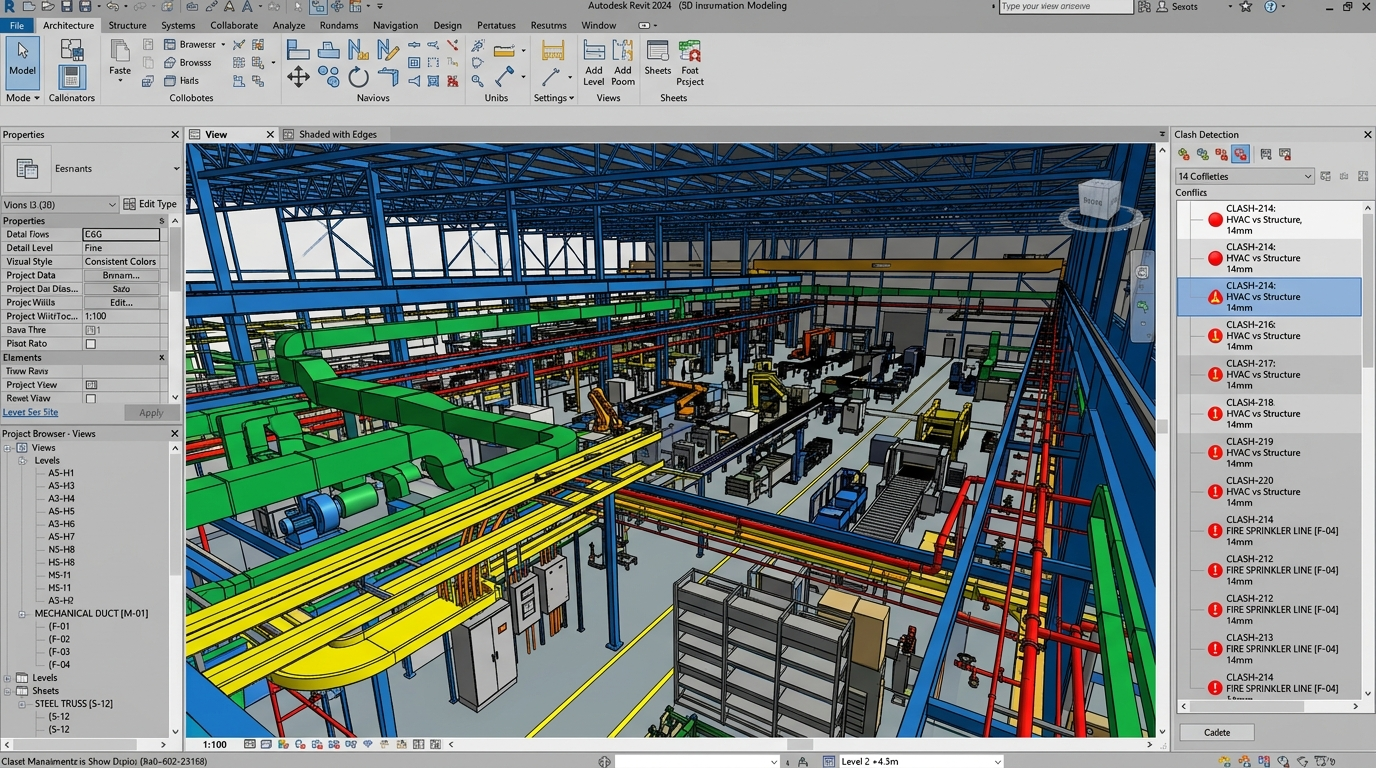
\includegraphics[width=186mm,height=55mm]{../../public/bim-model-3d.jpg}
  };
  \node[
    anchor=south, fill=TTCBlue!95!black, draw=TTCCyan!80!white,
    line width=0.6pt, text=white, rounded corners=4pt, inner sep=3.5pt,
    text width=160mm, align=center
  ] at ([yshift=2mm]bimimg.south) {
    {\fontsize{7.5}{9}\selectfont\bfseries\color{white} MÔ HÌNH SỐ HÓA BIM 3D/4D/5D TÍCH HỢP TOÀN DIỆN KẾT CẤU THÉP, MÓNG \& CƠ ĐIỆN MEP}
  };
\end{tikzpicture}
\end{minipage}

\newpage

% ============================================================
% TRANG 9: CÔNG TRÌNH XANH & TIÊU CHUẨN ESG
% ============================================================
\pageheaderbar{ĐỊNH HƯỚNG CÔNG TRÌNH XANH \& TIÊU CHUẨN ESG}{Trang 09}
\pagefooterbar{Trang 09}

\begin{minipage}[t][252mm]{\textwidth}
\secbrand{Giải Pháp Công Trình Xanh \& Tiêu Chuẩn Phát Triển Bền Vững ESG}{Sustainable Green Industrial Facilities, Low-Carbon Solutions \& ESG Standards}

% ESG Banner
\noindent
\begin{tikzpicture}
  \node[
    rounded corners=6pt, fill=TTCLightBlue, draw=TTCBorder, line width=0.8pt,
    minimum width=186mm, inner sep=7pt, text width=176mm, align=left
  ] {
    {\fontsize{9.5}{11.5}\selectfont\bfseries\color{TTCBlue} \faLeaf\quad CAM KẾT CHUẨN MỰC ESG CÙNG CHỦ ĐẦU TƯ FDI TOÀN CẦU}\\[2.5pt]
    {\fontsize{8}{12}\selectfont\color{TTCTextDark}
    TTC đồng hành cùng các tập đoàn đa quốc gia kiến tạo tổ hợp nhà máy phát thải thấp, tiết kiệm năng lượng và sẵn sàng đạt chứng chỉ công trình xanh quốc tế. Trong bối cảnh các nhà nhập khẩu lớn tại EU, Mỹ và Nhật Bản yêu cầu báo cáo Carbon Footprint trên chuỗi cung ứng, lựa chọn nhà xưởng xanh ESG-ready là lợi thế cạnh tranh sống còn.}
  };
\end{tikzpicture}

\vspace{2mm}

% 4 ESG Cards (2x2) -- 44mm height
\noindent
\begin{tabular}{@{}p{91mm}@{\hspace{4mm}}p{91mm}@{}}
  \begin{tikzpicture}
    \node[rounded corners=6pt, fill=white, draw=TTCBorder, line width=0.8pt, minimum width=91mm, minimum height=44mm, inner sep=6pt, align=left, text width=84mm] {
      {\fontsize{9.5}{11.5}\selectfont\bfseries\color{TTCBlue} \faAward\ CHỨNG NHẬN LEED, LOTUS \& EDGE}\\[3pt]
      {\fontsize{7.8}{11.2}\selectfont\color{TTCTextDark}
      Tư vấn quy hoạch và lập hồ sơ kỹ thuật đáp ứng các tiêu chuẩn công trình xanh quốc tế: \textbf{LEED (Mỹ)}, \textbf{LOTUS (Việt Nam)}, \textbf{EDGE (IFC/World Bank)} từ giai đoạn thiết kế cơ sở. Hỗ trợ đánh giá năng lượng và nước để đạt điểm tối ưu.}
    };
  \end{tikzpicture}
  &
  \begin{tikzpicture}
    \node[rounded corners=6pt, fill=white, draw=TTCBorder, line width=0.8pt, minimum width=91mm, minimum height=44mm, inner sep=6pt, align=left, text width=84mm] {
      {\fontsize{9.5}{11.5}\selectfont\bfseries\color{TTCBlue} \faRecycle\ VẬT LIỆU LOW-CARBON \& CÁCH NHIỆT}\\[3pt]
      {\fontsize{7.8}{11.2}\selectfont\color{TTCTextDark}
      Panel Rockwool chống cháy 2 giờ, tôn phản xạ nhiệt Solar Reflex và tấm lấy sáng Polycarbonate giảm nhiệt độ xưởng 5--8°C, \textbf{tiết kiệm 20\% điện năng} điều hòa. Sơn phủ Jotun Low-VOC bảo vệ sức khỏe công nhân và giảm khí thải hữu cơ.}
    };
  \end{tikzpicture}
  \\[2mm]
  \begin{tikzpicture}
    \node[rounded corners=6pt, fill=white, draw=TTCRed!80!white, line width=0.9pt, minimum width=91mm, minimum height=44mm, inner sep=6pt, align=left, text width=84mm] {
      {\fontsize{9.5}{11.5}\selectfont\bfseries\color{TTCRed} \faSun\ KẾT CẤU MÁI SẴN SÀNG ĐIỆN MẶT TRỜI}\\[3pt]
      {\fontsize{7.8}{11.2}\selectfont\color{TTCTextDark}
      Tính toán và gia cường trước tải trọng tĩnh cho toàn bộ hệ vì kèo (Solar Ready), sẵn sàng lắp đặt pin năng lượng mặt trời áp mái \textbf{1MWp -- 5MWp}. Hệ số hoàn vốn 4--6 năm, giảm chi phí điện vận hành 30--40\% và đóng góp chứng chỉ REC (Renewable Energy Certificate).}
    };
  \end{tikzpicture}
  &
  \begin{tikzpicture}
    \node[rounded corners=6pt, fill=white, draw=TTCBorder, line width=0.8pt, minimum width=91mm, minimum height=44mm, inner sep=6pt, align=left, text width=84mm] {
      {\fontsize{9.5}{11.5}\selectfont\bfseries\color{TTCBlue} \faTint\ TUẦN HOÀN NƯỚC \& XỬ LÝ CHẤT THẢI}\\[3pt]
      {\fontsize{7.8}{11.2}\selectfont\color{TTCTextDark}
      Hệ thống thu gom nước mưa tưới cây xanh, xử lý nước thải công nghiệp đạt \textbf{Cột A QCVN 40:2011} trước khi xả thải. Phân loại và tái chế 100\% phế liệu xây dựng (thép, gỗ, bê tông). Cam kết kiểm toán năng lượng và nước hàng năm.}
    };
  \end{tikzpicture}
\end{tabular}

\vspace{2mm}

% ESG Factory Image
\noindent
\begin{tikzpicture}
  \node[
    rounded corners=6pt, draw=TTCBorder, line width=0.8pt, inner sep=0pt, fill=white
  ] (esgimg) {
    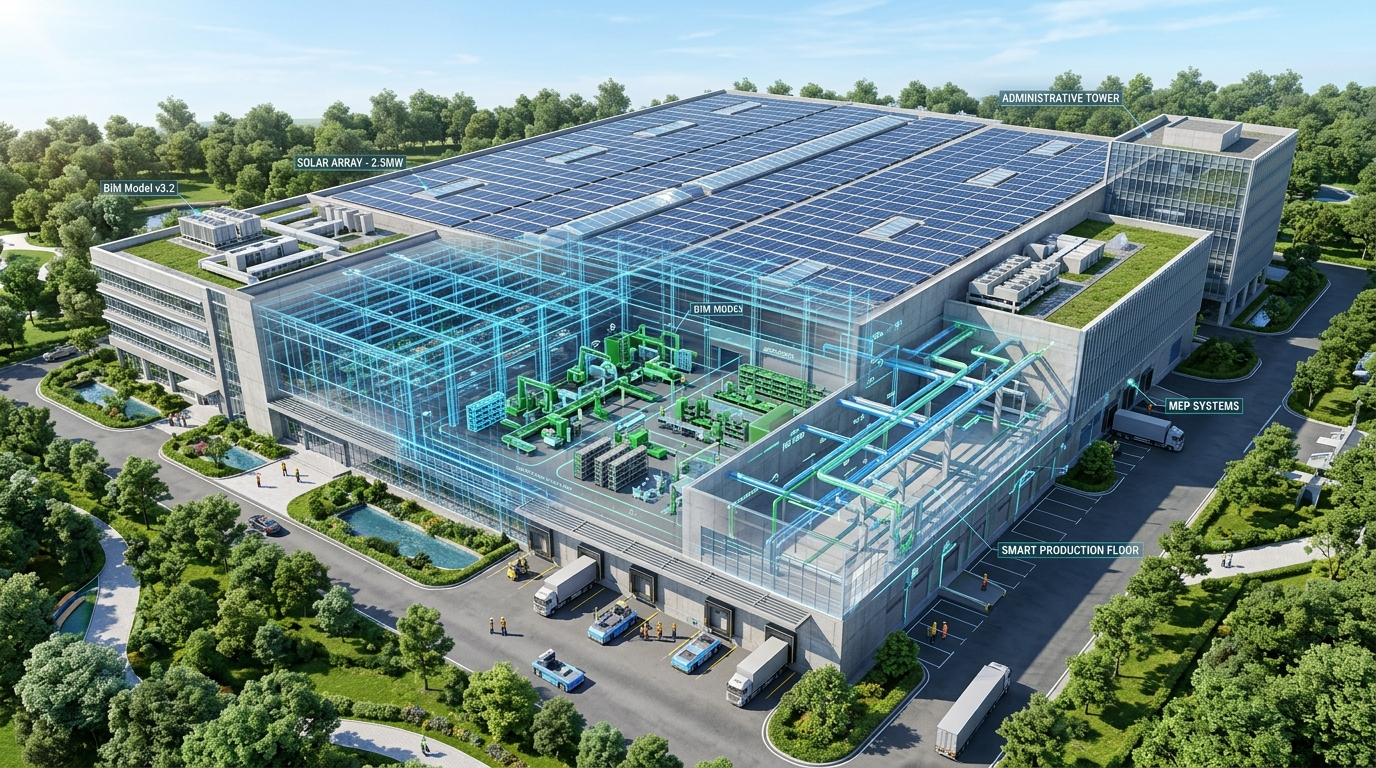
\includegraphics[width=186mm,height=55mm]{../../public/bim-esg-factory-3d.jpg}
  };
  \node[
    anchor=south, fill=TTCBlue!95!black, draw=TTCCyan!80!white,
    line width=0.6pt, text=white, rounded corners=4pt, inner sep=3.5pt,
    text width=160mm, align=center
  ] at ([yshift=2mm]esgimg.south) {
    {\fontsize{7.5}{9}\selectfont\bfseries\color{white} TỔ HỢP NHÀ XƯỞNG CÔNG NGHIỆP XANH ĐẠT TIÊU CHUẨN ESG -- TỐI ƯU ÁNH SÁNG \& NĂNG LƯỢNG MẶT TRỜI}
  };
\end{tikzpicture}
\end{minipage}

\newpage

% ============================================================
% TRANG 10: HỆ THỐNG KIỂM SOÁT CHẤT LƯỢNG & AN TOÀN HSE
% ============================================================
\pageheaderbar{HỆ THỐNG QUẢN LÝ CHẤT LƯỢNG QA/QC \& AN TOÀN HSE}{Trang 10}
\pagefooterbar{Trang 10}

\begin{minipage}[t][252mm]{\textwidth}
\secbrand{Hệ Thống Kiểm Soát Chất Lượng QA/QC \& An Toàn Tuyệt Đối HSE}{Quality Assurance/Quality Control Protocols \& Zero-Accident HSE Policy}

% 2 Columns: QA/QC vs HSE -- increased height to 110mm
\noindent
\begin{tabular}{@{}p{91mm}@{\hspace{4mm}}p{91mm}@{}}
  \begin{tikzpicture}
    \node[
      rounded corners=6pt, fill=white, draw=TTCBlue!60!white, line width=1pt,
      minimum width=91mm, minimum height=110mm, inner sep=7pt, align=left, text width=84mm
    ] {
      {\fontsize{10}{12}\selectfont\bfseries\color{TTCBlue} \faCheckDouble\quad QUY TRÌNH QA/QC 5 BƯỚC}\\[4pt]
      {\fontsize{7.8}{11.5}\selectfont\color{TTCTextDark}
      \textbf{1. Kiểm soát Vật liệu Đầu vào (MTC \& CO/CQ):}\newline
      100\% Thép Q345B/A572, bulong cường độ cao 8.8/10.9, bê tông thương phẩm có kết quả kéo nén từ phòng Lab Las-XD. Không nhập bất kỳ vật tư nào thiếu CO/CQ.\\[3pt]
      \textbf{2. Kiểm định Siêu âm Mối hàn AWS D1.1:}\newline
      100\% mối hàn chịu lực của dầm cột thép kiểm tra siêu âm (UT) và hạt từ tính (MT) bởi chuyên gia NDT độc lập có chứng chỉ ASNT Level II.\\[3pt]
      \textbf{3. Trắc đạc Laser Leica (Sai số $< \pm 2$mm):}\newline
      Đo đạc tim trục, độ võng xà gồ và độ thẳng đứng cột bằng máy toàn đạc Leica TS16, đảm bảo sai số lắp dựng tuyệt đối.\\[3pt]
      \textbf{4. Nghiệm thu ITP Chuyển bước:}\newline
      Hồ sơ ITP chi tiết từng công đoạn, dưới giám sát \& xác nhận Tư vấn Giám sát quốc tế. Mỗi Hold Point phải được ký duyệt trước khi chuyển bước.\\[3pt]
      \textbf{5. Kéo nén thí nghiệm tại hiện trường:}\newline
      Đúc mẫu bê tông 150x150mm, kéo nén 7 ngày \& 28 ngày tại Lab đạt chuẩn TCVN, đảm bảo cường độ R28 theo thiết kế.}
    };
  \end{tikzpicture}
  &
  \begin{tikzpicture}
    \node[
      rounded corners=6pt, fill=white, draw=TTCRed!80!white, line width=1pt,
      minimum width=91mm, minimum height=110mm, inner sep=7pt, align=left, text width=84mm
    ] {
      {\fontsize{10}{12}\selectfont\bfseries\color{TTCRed} \faShield*\quad CHÍNH SÁCH ZERO HSE 5 TRỤ CỘT}\\[4pt]
      {\fontsize{7.8}{11.5}\selectfont\color{TTCTextDark}
      \textbf{1. Toolbox Meeting 15 phút đầu ca:}\newline
      100\% kỹ sư \& công nhân học ATLĐ, cấp thẻ an toàn, phổ biến mối nguy và biện pháp xử lý theo từng công việc cụ thể trong ca.\\[3pt]
      \textbf{2. Trang bị Bảo hộ Chuẩn Châu Âu (PPE):}\newline
      Mũ cứng 3M, giày mũi thép Jogger, dây an toàn 2 móc Petzl chống rơi ngã, lưới an toàn bao quanh chu vi lắp dựng trên cao.\\[3pt]
      \textbf{3. Kiểm định 100\% Thiết bị Cẩu nâng:}\newline
      Cẩu tự hành, xe Boomlift, giàn giáo Ringlock có chứng chỉ kiểm định an toàn kỹ thuật còn hiệu lực. Cấm sử dụng thiết bị hết hạn.\\[3pt]
      \textbf{4. Ứng phó Khẩn cấp \& Diễn tập PCCC:}\newline
      Đội sơ cấp cứu hiện trường, diễn tập phương án PCCC cứu hộ phối hợp Ban Quản lý KCN định kỳ hàng quý.\\[3pt]
      \textbf{5. Camera AI Giám sát PPE 24/7:}\newline
      Hệ thống camera nhận diện tự động cảnh báo công nhân không đeo PPE, xâm nhập vùng nguy hiểm và vi phạm an toàn lao động.}
    };
  \end{tikzpicture}
\end{tabular}

\vspace{2mm}

% HSE Zero Accident KPI Banner
\noindent
\begin{tikzpicture}
  \node[
    rounded corners=6pt, fill=TTCDeepNavy!95!black, draw=TTCCyan!80!white, line width=1pt,
    text=white, minimum width=186mm, minimum height=26mm, inner sep=4pt
  ] {
    \begin{tabularx}{176mm}{@{}Y|Y|Y|Y|Y@{}}
      {\fontsize{15}{17}\selectfont\bfseries\color{TTCRed} 0\%} &
      {\fontsize{15}{17}\selectfont\bfseries\color{TTCCyan} 100\%} &
      {\fontsize{15}{17}\selectfont\bfseries\color{white} 100\%} &
      {\fontsize{15}{17}\selectfont\bfseries\color{TTCRed} 24/7} &
      {\fontsize{15}{17}\selectfont\bfseries\color{TTCCyan} ASNT II} \\
      {\fontsize{7}{8.5}\selectfont Tai nạn LĐ} &
      {\fontsize{7}{8.5}\selectfont Vật liệu CO/CQ} &
      {\fontsize{7}{8.5}\selectfont Thẻ An toàn} &
      {\fontsize{7}{8.5}\selectfont Giám sát HSE} &
      {\fontsize{7}{8.5}\selectfont Chứng chỉ NDT}
    \end{tabularx}
  };
\end{tikzpicture}

\vspace{2mm}

% Additional QA/QC info box
\noindent
\begin{tikzpicture}
  \node[
    rounded corners=6pt, fill=TTCLightBlue, draw=TTCBorder, line width=0.8pt,
    minimum width=186mm, inner sep=6pt, text width=176mm, align=left
  ] {
    {\fontsize{9}{11}\selectfont\bfseries\color{TTCBlue} \faTasks\quad TIÊU CHUẨN NGHIỆM THU ÁP DỤNG THEO QUY ĐỊNH:}\\[2pt]
    {\fontsize{7.5}{10.5}\selectfont\color{TTCTextDark}
    \textbf{Kết cấu thép:} TCVN 170:2007 (Nghiệm thu kết cấu thép), AWS D1.1 (Hàn kết cấu). \textbf{Bê tông:} TCVN 4453:1995 (Nghiệm thu BT toàn khối). \textbf{Nền móng:} TCVN 9394:2012 (Đóng \& ép cọc). \textbf{Cơ điện:} TCVN 9207:2012 (Đặt thiết bị điện). \textbf{PCCC:} QCVN 06:2022/BXD, Nghị định 136/2020/NĐ-CP.}
  };
\end{tikzpicture}
\end{minipage}

\newpage

% ============================================================
% TRANG 11: DANH MỤC DỰ ÁN TIÊU BIỂU & CHUỖI CUNG ỨNG FDI
% ============================================================
\pageheaderbar{DANH MỤC DỰ ÁN TIÊU BIỂU \& CHUỖI CUNG ỨNG}{Trang 11}
\pagefooterbar{Trang 11}

\begin{minipage}[t][252mm]{\textwidth}
\secbrand{Danh Mục Đại Dự Án Tiêu Biểu \& Chuỗi Cung Ứng Top 1}{Flagship Project Portfolio \& Strategic Tier-1 FDI Supply Chain Ecosystem}

% 6 Projects Table
\noindent
\begin{tikzpicture}
  \node[
    rounded corners=6pt, fill=white, draw=TTCBlue!40!white, line width=0.8pt,
    minimum width=186mm, inner sep=6pt, text width=176mm, align=center
  ] {
    {\fontsize{9.5}{11.5}\selectfont\bfseries\color{TTCBlue} \faBuilding\quad DANH MỤC ĐẠI DỰ ÁN TIÊU BIỂU (CASE STUDIES)}\\[3pt]
    {\fontsize{7.8}{10.8}\selectfont
    \begin{tabularx}{\linewidth}{@{}p{38mm} p{26mm} p{26mm} p{32mm} X@{}}
      \toprule
      \textbf{Tên Dự án} & \textbf{Chủ đầu tư} & \textbf{Quy mô} & \textbf{Địa điểm} & \textbf{Gói thầu EPC} \\
      \midrule
      \textbf{NM Gạch Hồng Trang} & VN / Fast-track & \textbf{\color{TTCRed}100.000 m²} & Vĩnh Phúc & Tổng thầu EPC Toàn diện \\
      \textbf{May Sông Hồng 7} & May Sông Hồng & \textbf{\color{TTCRed}57.927 m²} & Nam Định & KCT thép \& Hạ tầng Xanh \\
      \textbf{Japfa Comfeed} & Japfa (Indonesia) & \textbf{\color{TTCRed}50.000 m²} & VP / Thái Bình & Silo \& Nhà xưởng CNC \\
      \textbf{Daeyun ST Vina} & Daeyun (Hàn Quốc) & \textbf{\color{TTCRed}20.000 m²} & KCN Bá Thiện 2 & Xưởng CK \& Cleanroom \\
      \textbf{Sumidenso Cable} & Sumitomo (Nhật) & \textbf{\color{TTCRed}15.015 m²} & Hậu Giang & Xưởng Dây cáp điện \\
      \textbf{Foxconn Bắc Ninh} & Foxconn (Đài Loan) & \textbf{\color{TTCRed}9.000 m²} & KCN Quế Võ & KCT thép Xưởng cao tầng \\
      \bottomrule
    \end{tabularx}}
  };
\end{tikzpicture}

\vspace{2mm}

% 4 Project Photos Grid
\noindent
\begin{tabular}{@{}p{43.5mm}@{\hspace{4mm}}p{43.5mm}@{\hspace{4mm}}p{43.5mm}@{\hspace{4mm}}p{43.5mm}@{}}
  \begin{tikzpicture}
    \node[rounded corners=4pt, draw=TTCBorder, line width=0.7pt, inner sep=0pt, fill=white] (p1) {
      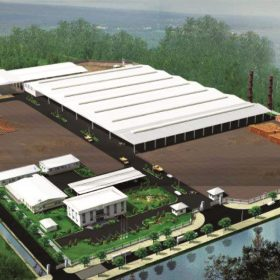
\includegraphics[width=43.5mm,height=28mm]{../../public/project-assets/hongtrang.jpg}
    };
    \node[anchor=south, fill=TTCBlue!95!black, text=white, rounded corners=2pt, inner sep=2pt, text width=40mm, align=center] at ([yshift=1.5mm]p1.south) {
      {\fontsize{6.5}{7.8}\selectfont\bfseries HỒNG TRANG (100K m²)}
    };
  \end{tikzpicture}
  &
  \begin{tikzpicture}
    \node[rounded corners=4pt, draw=TTCBorder, line width=0.7pt, inner sep=0pt, fill=white] (p2) {
      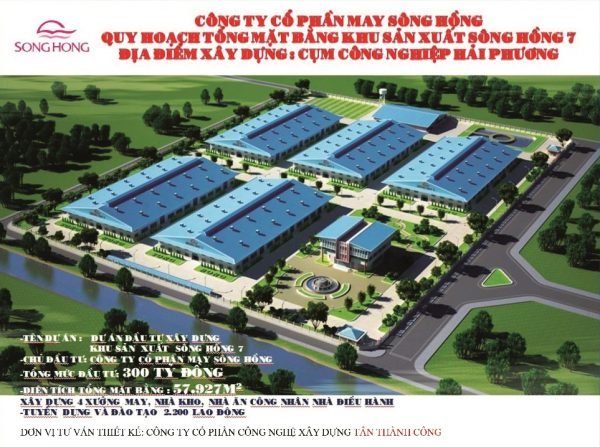
\includegraphics[width=43.5mm,height=28mm]{../../public/project-assets/songhong7.jpg}
    };
    \node[anchor=south, fill=TTCBlue!95!black, text=white, rounded corners=2pt, inner sep=2pt, text width=40mm, align=center] at ([yshift=1.5mm]p2.south) {
      {\fontsize{6.5}{7.8}\selectfont\bfseries SÔNG HỒNG 7 (58K m²)}
    };
  \end{tikzpicture}
  &
  \begin{tikzpicture}
    \node[rounded corners=4pt, draw=TTCBorder, line width=0.7pt, inner sep=0pt, fill=white] (p3) {
      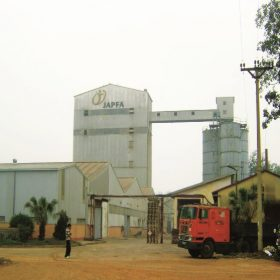
\includegraphics[width=43.5mm,height=28mm]{../../public/project-assets/japfa.jpg}
    };
    \node[anchor=south, fill=TTCBlue!95!black, text=white, rounded corners=2pt, inner sep=2pt, text width=40mm, align=center] at ([yshift=1.5mm]p3.south) {
      {\fontsize{6.5}{7.8}\selectfont\bfseries JAPFA (50K m²)}
    };
  \end{tikzpicture}
  &
  \begin{tikzpicture}
    \node[rounded corners=4pt, draw=TTCBorder, line width=0.7pt, inner sep=0pt, fill=white] (p4) {
      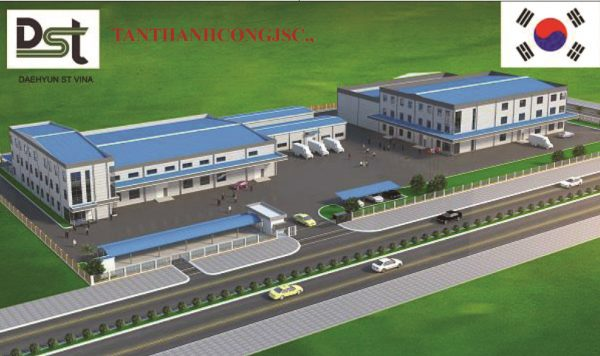
\includegraphics[width=43.5mm,height=28mm]{../../public/project-assets/daeyun.jpg}
    };
    \node[anchor=south, fill=TTCBlue!95!black, text=white, rounded corners=2pt, inner sep=2pt, text width=40mm, align=center] at ([yshift=1.5mm]p4.south) {
      {\fontsize{6.5}{7.8}\selectfont\bfseries DAEYUN (20K m²)}
    };
  \end{tikzpicture}
\end{tabular}

\vspace{2mm}

% Supply Chain Box -- expanded
\noindent
\begin{tikzpicture}
  \node[
    rounded corners=6pt, fill=TTCLightBlue, draw=TTCBorder, line width=0.8pt,
    minimum width=186mm, inner sep=7pt, text width=176mm, align=left
  ] {
    {\fontsize{9.5}{11.5}\selectfont\bfseries\color{TTCBlue} \faHandshake\quad CHUỖI CUNG ỨNG VẬT TƯ \& THIẾT BỊ TOP 1 (100\% CO/CQ)}\\[3pt]
    {\fontsize{7.8}{11.2}\selectfont\color{TTCTextDark}
    \textbf{Thép \& Tôn mái:} Hòa Phát Steel, Hoa Sen Group, Tôn Đông Á, BlueScope Lysaght, Pomina, Posco Vina.\\
    \textbf{Cơ điện \& Hóa chất:} Schneider Electric, Mitsubishi Electric, Panasonic, Grundfos, Dulux Professional, Jotun.\\
    \textbf{Bê tông \& Vật liệu:} Bê tông Hòa Phát, Xi măng Nghi Sơn, Vicostone, Panel Rockwool, Đá Granite Bình Định.}
  };
\end{tikzpicture}

\vspace{2mm}

% Project Stats Strip
\noindent
\begin{tikzpicture}
  \node[
    rounded corners=6pt, fill=TTCBlue, text=white,
    minimum width=186mm, minimum height=24mm, inner sep=4pt
  ] {
    \begin{tabularx}{176mm}{@{}Y|Y|Y|Y@{}}
      {\fontsize{15}{17}\selectfont\bfseries\color{TTCRed} >500.000 m²} &
      {\fontsize{15}{17}\selectfont\bfseries\color{TTCCyan} 150+} &
      {\fontsize{15}{17}\selectfont\bfseries\color{white} 100\%} &
      {\fontsize{15}{17}\selectfont\bfseries\color{TTCRed} 20+} \\
      {\fontsize{7.5}{9}\selectfont Diện tích sàn hoàn thành} &
      {\fontsize{7.5}{9}\selectfont Dự án FDI \& Trong nước} &
      {\fontsize{7.5}{9}\selectfont Đúng tiến độ bàn giao} &
      {\fontsize{7.5}{9}\selectfont Tỉnh thành thi công}
    \end{tabularx}
  };
\end{tikzpicture}

\vspace{2mm}

% Additional client testimonial / reference box
\noindent
\begin{tikzpicture}
  \node[
    rounded corners=6pt, fill=TTCDeepNavy!95!black, draw=TTCCyan!80!white, line width=0.8pt,
    minimum width=186mm, inner sep=7pt, text width=176mm, align=left
  ] {
    {\fontsize{9}{11}\selectfont\bfseries\color{TTCCyan} \faQuoteLeft\quad PHẢN HỒI TỪ CHỦ ĐẦU TƯ \& ĐỐI TÁC QUỐC TẾ:}\\[3pt]
    {\fontsize{7.8}{11}\selectfont\itshape\color{white}
    ``TTC là một trong số ít nhà thầu Việt Nam có khả năng đáp ứng đồng thời yêu cầu về tiến độ Fast-track, chất lượng kiểm soát nghiêm ngặt và tuân thủ an toàn lao động chuẩn quốc tế. Chúng tôi đánh giá cao cam kết bàn giao đúng hẹn và sự minh bạch tài chính xuyên suốt quá trình hợp tác.'' -- \textbf{Ban Quản lý Dự án, Tập đoàn Japfa Comfeed}}
  };
\end{tikzpicture}
\end{minipage}

\newpage

% ============================================================
% TRANG 12: BÌA SAU & THÔNG TIN LIÊN HỆ BAN GIÁM ĐỐC
% ============================================================
\thispagestyle{empty}
\null
\begin{tikzpicture}[remember picture,overlay]
  % Royal Deep Navy Background
  \fill[TTCDeepNavy] (current page.south west) rectangle (current page.north east);

  % Top Corner Geometric
  \fill[TTCBlue,opacity=0.85] (current page.north west) -- ++(80mm,0) -- ++(-80mm,-60mm) -- cycle;
  \fill[TTCRed,opacity=0.9] (current page.north east) -- ++(-60mm,0) -- ++(60mm,-45mm) -- cycle;
  \draw[TTCCyan,line width=2pt] (current page.north west) ++(80mm,0) -- ++(-80mm,-60mm);

  % Bottom Corner Geometric
  \fill[TTCBlue,opacity=0.85] (current page.south east) -- ++(-80mm,0) -- ++(80mm,60mm) -- cycle;
  \draw[TTCCyan,line width=2pt] (current page.south east) ++(-80mm,0) -- ++(80mm,60mm);
  \fill[TTCRed,opacity=0.9] (current page.south west) -- ++(60mm,0) -- ++(-60mm,45mm) -- cycle;

  % Title
  \node[anchor=west, text=white] at ([xshift=18mm, yshift=-26mm]current page.north west) {
    {\fontsize{22}{26}\selectfont\bfseries THÔNG TIN LIÊN HỆ \& HỢP TÁC}
  };
  \node[anchor=west, text=TTCCyan] at ([xshift=18mm, yshift=-36mm]current page.north west) {
    {\fontsize{10.5}{13}\selectfont\bfseries CONTACT INFORMATION \& INVESTMENT INQUIRIES}
  };
  \draw[TTCRed, line width=2.5pt]
    ([xshift=18mm, yshift=-42mm]current page.north west) --
    ([xshift=110mm, yshift=-42mm]current page.north west);

  % Company Title Card
  \node[
    anchor=west, fill=TTCBlue!95!TTCDeepNavy, draw=TTCCyan!80!white,
    line width=1pt, rounded corners=6pt, inner sep=10pt, text width=158mm
  ] at ([xshift=16mm, yshift=-65mm]current page.north west) {
    {\fontsize{12}{15}\selectfont\bfseries\color{white} CÔNG TY CỔ PHẦN CÔNG NGHỆ XÂY DỰNG TÂN THÀNH CÔNG}\\[2pt]
    {\fontsize{9.5}{12}\selectfont\bfseries\color{TTCCyan} TAN THANH CONG CONSTRUCTION TECHNOLOGY JOINT STOCK COMPANY}
  };

  % Contact Details Card
  \node[
    anchor=west, fill=TTCDeepNavy!95!black, draw=TTCBorder!40!white,
    line width=0.8pt, rounded corners=6pt, inner sep=12pt, text width=158mm
  ] at ([xshift=16mm, yshift=-128mm]current page.north west) {
    {\fontsize{10}{16}\selectfont\color{white}
    {\color{TTCRed}\faIdCard}\quad \textbf{Mã số thuế / MSDN:} 0107090447 (Cấp ngày 10/11/2015)\\[4.5pt]
    {\color{TTCRed}\faMapMarker*}\quad \textbf{Trụ sở ĐKKD:} Số 39, ngõ 292 đường Kim Giang, P. Đại Kim, Q. Hoàng Mai, Hà Nội\\[4.5pt]
    {\color{TTCRed}\faBuilding}\quad \textbf{Văn phòng giao dịch:} Số 19N7B, KĐT Trung Hòa Nhân Chính, Thanh Xuân, Hà Nội\\[4.5pt]
    {\color{TTCRed}\faUserTie}\quad \textbf{Đại diện pháp luật:} Ông PHẠM HUY TÂN -- Tổng Giám Đốc\\[4.5pt]
    {\color{TTCRed}\faPhone*}\quad \textbf{Hotline trực tiếp Ban Giám Đốc (24/7):} \textbf{\color{TTCCyan}+84 976 447 766}\\[4.5pt]
    {\color{TTCRed}\faEnvelope}\quad \textbf{Email:} info@tanthanhcongjsc.com \quad\textbar\quad contact@tanthanhcong.com.vn\\[4.5pt]
    {\color{TTCRed}\faGlobe}\quad \textbf{Website chính thức:} https://tanthanhcongjsc.com
    }
  };

  % Value Services Card
  \node[
    anchor=west, fill=TTCBlue!80!black, draw=TTCCyan!60!white,
    line width=0.8pt, rounded corners=6pt, inner sep=10pt, text width=158mm
  ] at ([xshift=16mm, yshift=-190mm]current page.north west) {
    {\fontsize{10.5}{13}\selectfont\bfseries\color{TTCRed} \faHandshake\quad CAM KẾT DỊCH VỤ DÀNH CHO CHỦ ĐẦU TƯ \& ĐỐI TÁC:}\\[3pt]
    {\fontsize{9}{13}\selectfont\color{white}
    \textbullet\ \textbf{Khảo sát mặt bằng \& Tư vấn quy hoạch:} Miễn phí trong vòng 24 giờ.\\[2pt]
    \textbullet\ \textbf{Báo giá \& Đề xuất tối ưu Value Engineering:} Hoàn thiện trong 48 giờ.\\[2pt]
    \textbullet\ \textbf{Hỗ trợ trọn gói thủ tục pháp lý:} IRC, ERC, Giấy phép Xây dựng, Thẩm duyệt PCCC.\\[2pt]
    \textbullet\ \textbf{Bảo hành công trình:} 24 tháng kết cấu, 12 tháng MEP, phản hồi sự cố trong 4 giờ.}
  };

  % Slogan
  \node[
    anchor=center, fill=TTCBlue!95!black, draw=TTCRed,
    line width=1pt, rounded corners=6pt, inner sep=8pt,
    text width=158mm, align=center
  ] at ([yshift=40mm]current page.south) {
    {\fontsize{12.5}{15}\selectfont\bfseries\color{white} ``TÂN THÀNH CÔNG -- \color{TTCRed}THÀNH CÔNG ĐỂ VƯƠN XA\color{white}''}\\[2pt]
    {\fontsize{9}{11.5}\selectfont\itshape\color{TTCCyan} Your Trusted General Contractor for Sustainable Industrial Facilities}
  };

  % Bottom Bar
  \fill[TTCRed] ([yshift=14mm]current page.south west) rectangle ([yshift=15.5mm]current page.south east);
  \node[anchor=center, text=white!60] at ([yshift=7mm]current page.south) {
    {\fontsize{7.5}{9}\selectfont \copyright\ 2026 Tân Thành Công Construction Technology JSC. All rights reserved. \quad\textbar\quad Bản quyền thuộc về TTC JSC}
  };
\end{tikzpicture}

\end{document}
